\documentclass[11pt]{elegantbook_2}
\usepackage{graphicx}
%\usepackage{float}
\definecolor{structurecolor}{RGB}{40,58,129}
\linespread{1.6}
\setlength{\footskip}{20pt}
\setlength{\parindent}{0pt}
\newcommand{\argmax}{\operatornamewithlimits{argmax}}
\newcommand{\argmin}{\operatornamewithlimits{argmin}}
\elegantnewtheorem{claim}{Claim}{prostyle}{Claim}
\DeclareMathOperator{\col}{col}
\title{Game Theory}
\author{Wenxiao Yang}
\institute{Haas School of Business, University of California Berkeley}
\date{2025}
\setcounter{tocdepth}{2}
\extrainfo{Mind offline, notes online.}

\cover{HZ.jpg}

% modify the color in the middle of titlepage
\definecolor{customcolor}{RGB}{250,255,240}
\colorlet{coverlinecolor}{customcolor}
\usepackage{cprotect}


\bibliographystyle{apalike_three}

\begin{document}
\maketitle

\frontmatter
\tableofcontents

\mainmatter




\chapter{Game Theory}
Based on
\begin{enumerate}[$\circ$]
    \item "Kreps, D. M., \& Sobel, J. (1994). Signalling. \textit{Handbook of game theory with economic applications}, 2, 849-867."
    \item Mas-Colell, Whinston, and Green, Microeconomic Theory, Oxford University Press (1995).
    \item UIUC ECON 530 21Fall, Nolan H. Miller
    \item UC Berkeley ECON 201A 23Fall, 201B 24Spring
    \item UC Berkeley MATH 272 23Fall, Alexander Teytelboym
    \item  Jehle, G., Reny, P.: Advanced Microeconomic Theory. Pearson, 3rd ed. (2011). Ch. 6.
    \item MIT 14.16 Strategy and Information, Mihai Manea
\end{enumerate}



\section{Basic Game Theory}
\subsection{Action and Domination Theorem}
Let $A$ be the finite set of possible actions and $\Omega$ be the finite set of possible states. A function can map the action and state to a value, $u(a,\omega)$. It can be represented by $\vec{u}(a)=\{u(a,\omega)\}_{\omega\in\Omega}$. It is common in game theory to assume the utility function is given or known.

A \textbf{mixed action} is a probability distribution over $A$, $\sigma\in\Delta(A)$.

A \textbf{belief} of the agent is a probability distribution over $\Omega$, $\mu\in\Delta(\Omega)$.

\begin{definition}[Optimal and Justifiable Mixed Action]
    %\normalfont
    A mixed action $\sigma\in\Delta(A)$ is \textbf{optimal} given $\mu\in\Delta(\Omega)$ if $$\mathbb{E}_\mu u(\sigma,\tilde{\omega})\geq \mathbb{E}_\mu u(\sigma',\tilde{\omega}),\ \forall \sigma'\in \Delta(A)$$
    A mixed action $\sigma\in\Delta(A)$ is \textbf{justifiable} if it is optimal for some belief $\mu\in\Delta(\Omega)$.
\end{definition}

\begin{definition}[Dominant and Dominated Action]
    %\normalfont
    A mixed action $\sigma\in\Delta(A)$ is \textbf{dominant} if $$u(\sigma,\omega)>u(\sigma',\omega),\ \forall \omega\in \Omega, \sigma'\in \Delta(A),\sigma\neq\sigma'$$
    A mixed action $\sigma\in\Delta(A)$ is \textbf{dominated} if $$u(\sigma,\omega)<u(\sigma',\omega),\ \forall \omega\in \Omega, \text{ and for some } \sigma'\in \Delta(A)$$
    In this case we say $\sigma'$ dominates $\sigma$.
\end{definition}

\begin{theorem}[Domination Theorem: Justifiable $=$ Not Dominated]
    A mixed action is justifiable \underline{if and only if} it is not dominated.
\end{theorem}
\begin{proof}
    $\Rightarrow$ is easily proved by the definition. We focus on proving $\Leftarrow$:
    
    Let $\mathcal{U}=\{\vec{u}(\sigma):\sigma\in\Delta(A)\}$ and $\sigma^*$ be an undominated mixed action. Then, we have $\mathcal{U}\cap(\{\vec{u}(\sigma^*)\}+\mathbb{R}_{++}^\Omega)=\emptyset$. Because $\mathcal{U}$ and $\{\vec{u}(\sigma^*)\}+\mathbb{R}_{++}^\Omega$ are disjoint, convex, and nonempty, we can use the Separating Hyperplane Theorem \ref{SHT}: $\exists p\in \mathbb{R}^\Omega,p\neq 0$ such that $p\cdot a\leq p\cdot b, \forall a\in\mathcal{U}, b\in (\{\vec{u}(\sigma^*)\}+\mathbb{R}_{++}^\Omega)$.

    \begin{claim}
        $p\cdot \vec{u}(\sigma)\leq p\cdot \vec{u}(\sigma^*), \forall \sigma\in\Delta(A)$.
    \end{claim}
    \begin{proof}
        For any positive number $m$, $\vec{u}(\sigma^*)+(\frac{1}{m},....,\frac{1}{m})\in \{\vec{u}(\sigma')\}+\mathbb{R}_{++}^\Omega$. So, for any $\sigma\in\Delta(A)$, $p\cdot \vec{u}(\sigma)\leq p\cdot\left(\vec{u}(\sigma^*)+(\frac{1}{m},....,\frac{1}{m})\right)$. By taking limit, $p\cdot \vec{u}(\sigma^*)=\lim_{m \rightarrow \infty}p\cdot\left(\vec{u}(\sigma^*)+(\frac{1}{m},....,\frac{1}{m})\right)\geq p\cdot \vec{u}(\sigma)$.
    \end{proof}
    \begin{claim}
        $p>0$.
    \end{claim}
    \begin{proof}
        Prove by the contradiction. Suppose $p_\omega<0$ for some $\omega\in\Omega$. Let $z=(\epsilon,...,\epsilon)+M\mathbb{1}_\omega, M>0,\epsilon>0$. So, $\vec{u}(\sigma^*)+z\in (\{\vec{u}(\sigma^*)\}+\mathbb{R}_{++}^\Omega)$. We have $p\cdot\vec{u}(\sigma^*)\leq p\cdot (\vec{u}(\sigma^*)+z)$ by the result of SHT. There is a contradiction since $p_\omega<0$. So, we have $p\geq 0$. Because $p\neq 0$, $p>0$ is proved.
    \end{proof}
    Finally, we normalize $p$ to $\mu=\frac{1}{\sum_{\omega}p_\omega}p$. Then, $\sigma^*$ is optimal for the belief $\mu$, which means $\sigma^*$ is justifiable.
\end{proof}










\subsection{Extensive Game}
\begin{definition}[History]
    %\normalfont
    The sequences of actions are called \textbf{histories}. $h'=(\underbrace{a_1,...,a_n}_{h: \text{prefix of }h'},a_{n+1},...)\in H$. We call $h'$ is the \textbf{continuation} of $h$. $h$ is a \textbf{terminal} of $H$ if there is no continuation of $h$ in $H$. ($\emptyset\in H$.)
\end{definition}

\begin{definition}[Extensive form Perfect Information Game]
    %\normalfont
    Am extensive form game with prefect information is defined as $G=\{N,A,H,Z,P,O,o,\succ_{n\in N}\}$, where $N$ is the set of players, $A$ is the set of actions, $H$ is the set of all histories, $Z$ is the set of all histories that are terminals, $P:H/Z \rightarrow N$ is a mapping from a non-terminal histories to a player (who moves after a non-terminal history), $O$ is the set of outcomes, and $o$ is a function from $Z$ to $O$.\\
    A PIG is \underline{finite horizon} if there is a bound on the length of its histories.
\end{definition}


We denote $A(h)$ as the actions available to player $P(h)$ after a history $h$.

Let $H_i=\{h\in H/Z:i=P(h)\}$ be the set of histories that player $i$ moves after.

\begin{definition}[Strategy]
    %\normalfont
    A \textbf{strategy} is defined as a function $s_i:H_i \rightarrow A$ for which $s_i(h)\in A(h),\forall h\in H_i$. Let $S_i$ be the set of all strategies available to the player $i$. A \textbf{strategy profile} is a collection of strategy $s=(s_i)_{i\in N}$.
\end{definition}



\begin{definition}[Subgame]
%\normalfont
    A \textbf{subgame} of a PIG $G=\{N,A,H,Z,P,O,o,\succ_{n\in N}\}$ is a game (a PIG) that starts after a given finite history $h\in H$. Formally, the subgame $G(h)$ associated with $h=(h_1,...,h_n)\in H$ is $G(h)=\{N,A,H_h,Z,P_h,O,o_h,\succ_{n\in N}\}$, where
    \begin{equation}
        \begin{aligned}
            H_h=\{(a_1,a_2,...):(h_1,...,h_n,a_1,a_2,...)\in H\}\\
            o_h(h')=o(hh'), P_h(h')=P(hh')
        \end{aligned}
        \nonumber
    \end{equation}
    A strategy $s$ of $G$ defines a strategy $s_h$ of $G(h)$ by $s_h(h')=s(hh')$.
\end{definition}

\begin{definition}[Subgame Perfect Equilibrium (SPNE)]
    %\normalfont
    A \textbf{subgame perfect equilibrium (SPNE)} of $G$ is a strategy profile $s^*$ such that for every subgame $G(h)$ it holds that $h^{\prime} \mapsto s_i^*\left(h h^{\prime}\right)$ is an optimal strategy in $G(h)$, given beliefs that the rest of the players behave according to $s_{-i}^*$ (or its restriction to $G(h)$).
\end{definition}

\begin{definition}[Profitable Deviation]
    %\normalfont
    Let $s$ be a strategy profile. We say that $s_i^{\prime}$ is a \textbf{profitable deviation} from $s$ for player $i$ at history $h$ if $s_i^{\prime}$ is a strategy for $G$ such that
    $$
    o_h\left(s_i^{\prime}, s_{-i}\right) \succ_i o_h(s)
    $$
\end{definition}
Note that a strategy profile has no profitable deviations iff it's a SPNE.

\begin{theorem}[The one-deviation principle]
    Let $G=\left(N, A, H, O, o, P,\left\{\preceq_i\right\}_{i \in N}\right)$ be a finite horizon, extensive form game with perfect information. Let $s$ be a strategy profile that is \underline{not} a subgame perfect equilibrium. There exists some history $h$ and a profitable deviation $\bar{s}_i$ for player $i=P(h)$ in $G(h)$ such that $\bar{s}_i(k)=s_i(k)$ for all $k \neq h$.
\end{theorem}
\begin{enumerate}[$\circ$]
    \item Let $G=\left(N, A, H, O, o, P,\left\{\preceq_i\right\}_{i \in N}\right)$ be a PIG.
    \item $A(\emptyset)$ is the set of allowed initial actions for player $i=P(\emptyset)$. For each $b \in A(\emptyset)$, let $s^{G(b)}$ be some strategy profile for the subgame $G(b)$.
    \item Given some $a \in A(\emptyset)$, we denote by $s^a$ the strategy profile for $G$ in which player $i=P(\emptyset)$ chooses the initial action $a$, and for each action $b \in A(\emptyset)$ the subgame $G(b)$ is played according to $s^{G(b)}$.
    \item So $s_i^a(\emptyset)=a$ and for every player $j, b \in A(\emptyset)$ and $b h \in H \backslash Z$, $s_j^a(b h)=s_j^{G(b)}(h)$.
\end{enumerate}
\begin{lemma}[Backward Induction]
    Let $G=\left(N, A, H, Z, O, o, P,\left\{\preceq_i\right\}_{i \in N}\right)$ be a finite PIG. Assume that for each $b \in A(\emptyset)$ the subgame $G(b)$ has a subgame perfect equilibrium $s^{G(b)}$. Let $i=P(\emptyset)$ and let $a$ be the $\succ_i$-maximizer over $A(\emptyset)$ of $o_a\left(s^{G(a)}\right)$. Then $s^a$ is a subgame perfect equilibrium of $G$.
\end{lemma}


\subsection{Strategic Form Game}
\begin{definition}[Normal Form Game]
    %\normalfont
    A game in \textbf{normal form} is denoted by $$G =\left(\underbrace{N}_{\textnormal{players}},\underbrace{\{S_i\}_{i\in N}}_{\textnormal{Strategy Set}},\underbrace{\{u_i(\cdot)\}_{i\in N}}_{\textnormal{VNM utility}}\right)$$

    $u_i:\prod_{i\in I}S_i \rightarrow \mathbb{R}$ is the utility function that maps all players' strategies to a player's utilities.

    A \underline{finite} game is a normal-form game in which the set of players $N$ is a finite set, and the set of strategy profiles $S$ is finite.
\end{definition}

\begin{definition}[Mixed/Pure Strategy]
%\normalfont
A mixed strategy  for player $i$ is a probability distribution $\sigma_i\in\Delta(S_i)$.\\
Elements of $S_i$ are called pure strategies.
\end{definition}

\begin{definition}[Dominant/Dominated Strategy]
    %\normalfont
    A strategy $\sigma_i\in \Delta(S_i)$ is a \textbf{dominant strategy} for $i$ in $G$, if we have $u_i(\sigma_i,\sigma_{-i})> u_i(\sigma'_i,\sigma_{-i}), \forall \sigma'_i\neq \sigma_i, \sigma_{-i}\in\times_{j\neq i}\Delta(S_j)$.\\
    A strategy $\sigma_i\in \Delta(S_i)$ is a \textbf{dominated strategy} for $i$ in $G$, if $\exists \sigma'_i\neq \sigma_i$, $u_i(\sigma_i,\sigma_{-i})<u_i(\sigma'_i,\sigma_{-i}), \forall \sigma_{-i}\in\times_{j\neq i}\Delta(S_j)$.\\
    A strategy $\sigma_i\in \Delta(S_i)$ is a \textbf{weakly dominated strategy} for $i$ in $G$, if $\exists \sigma'_i\neq \sigma_i$, $u_i(\sigma_i,\sigma_{-i})\leq u_i(\sigma'_i,\sigma_{-i}), \forall \sigma_{-i}\in\times_{j\neq i}\Delta(S_j)$ and there is a $\sigma_{-i}\in\times_{j\neq i}\Delta(S_j)$, $u_i(\sigma_i,\sigma_{-i})< u_i(\sigma'_i,\sigma_{-i})$
\end{definition}

\begin{lemma}
    1. A dominant strategy is always pure.\\
    2. A strategy $\sigma'_i$ dominates $\sigma_i$ iff $u_i(\sigma'_i,s_{-i})> u_i(\sigma_i,s_{-i})$, for all pure strategy profiles $s_{-i}\in S_{-i}$.
\end{lemma}


\begin{definition}[Belief, Best Response]
    %\normalfont
    A \textbf{belief} for player $i$ is a probability distribution $\mu\in\Delta(S_{-i})$.\\
    A strategy $\sigma_i \in \Delta(S_i)$ is the \textbf{best response} to beliefs $\mu$ if it solves the problem of $\max_{\sigma_i\in\Delta(S_i)}u_i(\sigma_i,s_{-i})$.\\
    Denote the set of all best responses to $\mu$ by $\beta_i(\mu)$.
\end{definition}
\begin{lemma}[Mixed Strategy is BR iff its Pure Strategies are Indifferent]
    A mixed strategy $\sigma_i$ is in $\beta_i(\mu)$ iff every pure strategy in the support of $\sigma_i$ is in $\beta_i(\mu)$. In particular, every strategy in the support of $\sigma_i$ yields the same payoff to $i$.
\end{lemma}

\begin{theorem}[Domination Theorem rephrased]
    In a finite game, a strategy is dominated iff there is no belief to which it is a best response.
\end{theorem}


\begin{definition}[Algorithm: Iterated Elimination of Dominated Strategies (IEDS)]
    %\normalfont
    Let $\left(N,\left(S_i\right),\left(u_i\right)\right)$ be a finite game; $N=[n]$.
    \begin{enumerate}[$\bullet$]
        \item We define (inductively) $n$ sequences of sets of mixed strategies.
        \item Let $D_i^0=\Delta\left(S_i\right)$.
        \item Given $D_1^{k-1}, \ldots, D_n^{k-1}$, let
        $$
        D_i^k=\left\{\sigma_i: \nexists \bar{\sigma}_i: u_i\left(\sigma_i, \sigma_{-i}\right)<u_i\left(\bar{\sigma}_i, \sigma_{-i}\right) \forall \sigma_{-i} \in \times_{j \neq i} D_j^{k-1}\right\} .
        $$
        \item Note that $\left\{D_i^k\right\}$ is a decreasing sequence of sets.
        \item Let $D_i = \cap_{k=0}^\infty D_i^k$.
        \item The set $D = \times_{i=1}^n D_i$ be the set of strategies that survive the iterated elimination of dominated strategies.
    \end{enumerate}
    A game is called \textbf{dominance-solvable} if $D$ is a singleton.
\end{definition}


\begin{definition}[Rationalizable Strategies]
%\normalfont
    \begin{enumerate}[$\bullet$]
        \item $R_i^0=\Delta\left(S_i\right)$.
        \item Given $R_1^{k-1}, \ldots, R_n^{k-1}$, Let
        $$
        \begin{aligned}
        & Z_i^k=\left\{s_i \in S_i: \sigma_i\left(s_i\right)>0 \text { for some } \sigma_i \in R_i^{k-1}\right\} \\
        & R_i^k=\left\{\sigma_i \in \Delta\left(S_i\right): \exists \mu \in \Delta\left(\times_{j \neq i} Z_j^k\right) \text { s.t. } \sigma_i \in \beta_i(\mu)\right\}
        \end{aligned}
        $$
    \end{enumerate}
    Note: $\left\{R_i^k\right\}_{k=0}^{\infty}$ is a decreasing sequence of sets.\\
    Let $R_i=\cap_{k=0}^{\infty} R_i^k$.\\
    The \textbf{rationalizable strategies} are the elements of $R=\times_{i=1}^n R_i$.
\end{definition}

\begin{lemma}
    In a finite game, $R$ is always non-empty and contains a pure strategy profile.
\end{lemma}

\begin{proposition}
    $\sigma_i \in \Delta(S_i)$ is \textbf{rationalizable} iff there are sets $Z_1,..., Z_n, Z_j \subseteq S_j$ such that
    \begin{enumerate}
        \item $\sigma_i \in \beta_i(\mu_i)$ for some $\mu_i \in \Delta(\times_{h\neq i}Z_h)$.
        \item for every $s_j \in Z_j$ there is $\mu_j \in \Delta(\times_{h\neq j}Z_h)$ such that $s_j\in \beta_j(\mu_j)$.
    \end{enumerate}
\end{proposition}

\begin{corollary}[Rationalizable = IEDS]
    Rationalizable strategies are exactly the strategies survive the iterated elimination of dominated strategies, $$R=D$$
\end{corollary}
















\subsection{Nash Equilibrium and Existence}
\begin{definition}[Nash Equilibrium]
    %\normalfont
    A strategy profile $\Sigma=(\sigma_1,...,\sigma_I)$ is a \textbf{Nash} equilibrium of the game $G$ if for every $i\in I$, we have: $u_i(\sigma^*_i,\sigma^*_{-i})\geq u_i(\sigma'_i,\sigma^*_{-i}), \forall \sigma'_i\in \Delta(S_i)$ (no profitable deviation). In other words,
    \begin{enumerate}
        \item $\sigma_i$ is the \underline{best response} to beliefs $\mu_i\in \Delta (S_{-i})$
        \item $\mu_i=\sigma_{-i}$ (correct beliefs).
    \end{enumerate}
\end{definition}
\begin{enumerate}
    \item In rationalizable strategies, beliefs can be incorrect.
    \item In a Nash equilibrium, beliefs are correct. Any strategy in a Nash equilibrium is rationalizable.
\end{enumerate}

\begin{definition}[Best Response Correspondence]
    %\normalfont
    In a Nash equilibrium the player $i$'s best response correspondence $\beta_i:\Delta(S_{-i})\rightarrow 2^{\Delta(S_i)}$ is defined as $\beta_i(\sigma_{-i})=\arg\max_{\sigma_i\in\Delta(S_i)}u_i(\sigma_i,\sigma_{-i})$. Let $\beta(\sigma)=\times_{i\in I}\beta_i(\sigma_{-i})$. Then $\sigma$ is a Nash equilibrium iff $\beta(\sigma)=\sigma$. $\beta$ is called the \textbf{best response correspondence} of the game.
\end{definition}

\begin{theorem}[Existence of Nash Equilibrium]
    A Nash equilibrium exists in a finite game $\Gamma$, if for all $i\in I$,
    \begin{enumerate}[(i).]
        \item $S_i$ is non-empty, convex, compact, subset of $\mathbb{R}^m$ (i.e., for some finite dimensions of real numbers).
        \item $u_i(s_i,...,s_I)$ is continuous in $(s_i,...,s_I)$ and quasi-concave in any $s_i$.
    \end{enumerate}
\end{theorem}
\begin{proof}
    We prove a lemma for the best response correspondence $\beta_i(s_{-i})=\argmax_{s_i\in S_i}u(s_i,s_{-i})$ firstly.
    \begin{lemma}
        Suppose $\{S_i\}_{i\in I}$ are non-empty. Suppose that $S_i$ is compact and convex and $u_i$ is continuous in $(s_i,...,s_I)$ and quasi-concave in any $s_i$, then best response correspondence $\beta_i(s_{-i})$ is non-empty, convex-valued and uhc.
    \end{lemma}
    \begin{proof}
        This lemma is proved by Berge's Maximum Theorem (Theroem \ref{thm:Berge's Maximum Theorem}).
    \end{proof}
    Consider the best response correspondence of the game $\beta$ with $\beta(s_i,...,s_I)=\{\beta_1(s_{-1}),...,\beta_I(s_{-I})\}$.

    As we proved $\beta$ is non-empty, convex-valued and uhc from $S$ to $S$ where $S$ is non-empty, compact, and convex. By the Kakutani's Fixed Point Theorem (Theorem \ref{thm:Kakutani's Fixed Point Theorem}), we have $\beta$ has a fixed point $s\in S$, which should be the Nash equilibrium.
\end{proof}

\subsection{Bayesian Game}
\begin{definition}[Bayesian Game]
    %\normalfont
    A \textbf{Bayesian game} is defined by $$\Gamma=(I, \Omega, \{A_i\}_{i\in I}, \{u_i(\cdot)\}_{i\in I},\{\Theta_i\}_{i\in I}, \{F_i\}_{i\in I})$$
    where $\Omega$ is the state space, $u_i:A\times \Omega$ is $i$'s payoff function, and $F_i\in\Delta\left(\Omega\times\Theta_i\right)$ is the (prior) distribution of the player $i$'s type.
\end{definition}

\begin{definition}[Normal-form Bayesian game]
    %\normalfont
    Assume a finite game. The \textbf{normal-form game} can be represented by $$\left(I,(S_i,U_i)_{i\in I}\right)$$ defined by letting $S_i$ be the set of strategies based on types $s_i:\Theta_i \rightarrow A_i$ and
    \begin{equation}
        \begin{aligned}
            U_i(s)=\sum_{\omega\in\Omega}\sum_{(\theta_i)_{i\in I}\in \Theta}p(\omega,\theta_1,...,\theta_I)u_i(s_1(\theta_1),..., s_I(\theta_I),\omega)
        \end{aligned}
        \nonumber
    \end{equation}
    for all $s\in S$.

    A \textbf{Bayesian Nash equilibrium} (BNE) of a Bayesian game is a strategy profile $(s_1,...,s_n)$ that is a Nash equilibrium of the derived normal-form game.
\end{definition}

\begin{definition}[Best Response, Interim Payoff]
    %\normalfont
    $s_i$ is a BR to $s_{-i}$ iff for all $\theta_i$, $s_i(\theta_i)$ maximizes the \textbf{interim payoff} of player $i$. The interim payoff is defined by the expected payoff given the type $\theta_i$ of player $i$ by playing action $a_i$.
    \begin{equation}
        \begin{aligned}
            \mathbb{E}_{\omega\in\Omega,\tilde{\theta}_{-i}\in\Theta_{-i}}[u_i(a_i,s_{-i}(\tilde{\theta}_{-i}),\omega)|\theta_i]
        \end{aligned}
        \nonumber
    \end{equation}
\end{definition}

\subsection{Zero-sum Game}
Let $G=(\{1,2\},(S_1,S_2),(u_1,u_2))$. Suppose there is a constant $c$ so that $u_1(s)+u_2(s)=c, \forall s\in S$. Then $G$ is equivalent to a zero-sum game.

\begin{definition}[Saddle Point]
    %\normalfont
    Let $X,Y$ be sets and $f:X\times Y \rightarrow \mathbb{R}$ a real function. $(x^*,y^*)\in X\times Y$ is a \textbf{saddle point} of $f$ if $x^*\in\argmax_{x\in X}f(x,y^*)$ and $y^*\in\argmin_{y\in Y}f(x^*,y)$. That is,
    \begin{equation}
        \begin{aligned}
            f(x,y^*)\leq f(x^*,y^*)\leq f(x^*,y),\forall x\in X,y\in Y
        \end{aligned}
        \nonumber
    \end{equation}
\end{definition}

Consider a zero-sum game of two players. The strategy of the player 1 is max-min strategy, which is given by
\begin{equation}
    \begin{aligned}
        \max_{\sigma_1}\min_{\sigma_2}u(\sigma_1,\sigma_2)
    \end{aligned}
    \nonumber
\end{equation}
and the strategy of the player 2 is min-max strategy, which is given by
\begin{equation}
    \begin{aligned}
        \min_{\sigma_2}\max_{\sigma_1}u(\sigma_1,\sigma_2)
    \end{aligned}
    \nonumber
\end{equation}
\begin{proposition}[min-max$\geq$max-min]
    Min-max strategy is always better than max-min strategy. That is,
    \begin{equation}
        \begin{aligned}
            \max_{\sigma_1}\min_{\sigma_2}u(\sigma_1,\sigma_2)\leq \min_{\sigma_2}\max_{\sigma_1}u(\sigma_1,\sigma_2)
        \end{aligned}
        \nonumber
    \end{equation}
\end{proposition}
\begin{proof}
    As $u(\sigma_1',\sigma_2)\leq \max_{\sigma_1}u(\sigma_1,\sigma_2)$ for all $\sigma_1'$, we have
    \begin{equation}
        \begin{aligned}
            \min_{\sigma_2}u(\sigma_1',\sigma_2)&\leq \min_{\sigma_2}\max_{\sigma_1}u(\sigma_1,\sigma_2),\forall \sigma_1'\\
            \Rightarrow \max_{\sigma_1}\min_{\sigma_2}u(\sigma_1,\sigma_2)&\leq \min_{\sigma_2}\max_{\sigma_1}u(\sigma_1,\sigma_2)
        \end{aligned}
        \nonumber
    \end{equation}
\end{proof}
We shall prove that these are in fact equal in the zero-sum game.

\begin{definition}[Value of a zero-sum game]
    %\normalfont
    A \textbf{value} for a zero-sum game $G$ is a number $v \in \mathbb{R}$ for which there exists a strategy profile $\left(\bar{\sigma}_1, \bar{\sigma}_2\right)$ such that
    $$
    \begin{matrix}u\left(\bar{\sigma}_1, \sigma_2\right) \geq v & \text { for all } \sigma_2 \\ u\left(\sigma_1, \bar{\sigma}_2\right) \leq v & \text { for all } \sigma_1\end{matrix}
    $$
\end{definition}
Note: $v=u\left(\bar{\sigma}_1, \bar{\sigma}_2\right)$.
The value is unique (if its exists), and represents a guaranteed payoff for the players.
(Uniqueness: Suppose there are two values, $v$ and $v^{\prime}>v$, achieved by profiles $\sigma$ and $\sigma^{\prime}$. Then when 2 plays $\sigma_2$ we have that $u\left(\sigma_1^{\prime}, \sigma_2\right) \geq v^{\prime}$ because $\sigma_1^{\prime}$ guarantees $v^{\prime}$. And when 1 plays $\sigma_1^{\prime}$ we have $v \geq u\left(\sigma_1^{\prime}, \sigma_2\right)$ because $\sigma_2$ guarantees $v$. So $v^{\prime}>v$ leads to a contradiction.)

\begin{proposition}
    The following statements are equivalent
    \begin{enumerate}
        \item $\left(\bar{\sigma}_1, \bar{\sigma}_2\right)$ is a Nash equilibrium.
        \item $v=u\left(\bar{\sigma}_1, \bar{\sigma}_2\right)$.
    \end{enumerate}
\end{proposition}


\begin{corollary}
    If $\left(\sigma_1^*, \sigma_2^*\right)$ and $\left(\bar{\sigma}_1, \bar{\sigma}_2\right)$ are Nash equilibria of $G$, then so are the profiles $\left(\bar{\sigma}_1, \sigma_2^*\right)$ and $\left(\sigma_1^*, \bar{\sigma}_2\right)$.
\end{corollary}

\begin{theorem}[Minimax Theorem]
    Let $G$ be a zero-sum game. There is a strategy profile $(\sigma_1^*, \sigma_2^*)$ s.t.
    \begin{equation}
        \begin{aligned}
            \max_{\sigma_1}\min_{\sigma_2}u(\sigma_1,\sigma_2)=v= \min_{\sigma_2}\max_{\sigma_1}u(\sigma_1,\sigma_2)
        \end{aligned}
        \nonumber
    \end{equation}
    where $v=u(\sigma_1^*, \sigma_2^*)$ is the value of the game and $(\sigma_1^*, \sigma_2^*)$ is a Nash equilibrium.
\end{theorem}
\begin{proof}
    Let $n_i=|S_i|$. Let $\vec{u}(\sigma_2):=\{u(s_1,\sigma_2):s_1\in S_1\}$. Let $\mathbb{C}=\{\vec{u}(\sigma_2):\sigma_2\in \Delta(S_2)\}$. We can find $\mathbb{C}$ is convex and compact.

    Let $m(x):=\max\{x_i:i=1,...,n_1\}$. Then, the player 2's min max payoff is given by $v:=\inf\{m(x):x\in \mathbb{C}\}$. By compactness, exists strategy $\sigma_2^*$ such that $\vec{u}(\sigma_2^*)=(v,v,...,v)$. That is, $u(s_1,\sigma_2^*)=v,\forall s_1\in S_1$.

    Let $\mathbb{A}:=\{z\in \mathbb{R}^{n_1}:z<<(v,v,...,v)\}=(v,v,...,v)-\mathbb{R}^{n_1}_{++}$. As $\mathbb{C}$ and $\mathbb{A}$ are disjoint. By SHT, we can find a $p\neq 0$ s.t. $p\cdot \mathbb{A}\leq p\cdot \mathbb{C}$. $p>0$ since $\mathbb{A}$ can have arbitrary small elements in any dimension. Then, we normalize $p$ to be in $\Delta(S_1)$, denote it by $\sigma^*_1$.

    By limitation, $v=\sigma^*_1\cdot(v,v,...,v)=\lim_{\epsilon \rightarrow 0^+}\sigma^*_1\cdot (v-\epsilon,v-\epsilon,...,v-\epsilon)\leq \sigma^*_1\cdot\vec{u}(\sigma_2),\forall \sigma_2\in \Delta(S_2)$.

    Hence, $u(s_1,\sigma_2^*)\leq m(\vec{u}(\sigma_2^*))=v=u(\sigma_1^*,\sigma_2^*)\leq u(\sigma_1^*,\sigma_2)$
\end{proof}

\subsection{Correlated equilibrium}
Suppose there is a mediator that give advices to each player based on a distribution $p \in \Delta(S)$. A player doesn't know other players' advices but knows the distribution $p$.
\begin{definition}[Correlated Equilibrium]
    %\normalfont
    A \textbf{correlated equilibrium} of $G$ is any probability distribution $p \in \Delta(S)$ such that, for all $i$ and $s_i,s'_i \in S_i$, the player $i$ can't get a higher expected profit than by following the advice,
    \begin{equation}
        \begin{aligned}
            \sum_{s_{-i}\in S_{-i}}p(s_i,s_{-i})u_i(s_i,s_{-i})\geq\sum_{s_{-i}\in S_{-i}}p(s_i,s_{-i})u_i(s'_i,s_{-i})
        \end{aligned}
        \nonumber
    \end{equation}
    where LHS is the expected profit of player $i$ when he receives an advice $s_i$ from the mediator.
\end{definition}

Let $G$ be a finite game,
\begin{proposition}
    If we identify a Nash equilibrium $\sigma$ of $G$ with a probability distribution on $\Delta(S)$, then any Nash equilibrium of $G$ is also a correlated equilibrium.
\end{proposition}

\begin{proposition}
    The set of correlated equilibria is a non-empty, convex, compact subset of $\Delta(S)$.
\end{proposition}

For $p\in\Delta(S)$, the \textbf{marginal distribution} on $S_i$ is given by
\begin{equation}
    \begin{aligned}
        p_i(s_i)=\sum_{s_{-i}\in S_{-i}}p(s_i,s_{-i})
    \end{aligned}
    \nonumber
\end{equation}
\begin{proposition}
    A correlated equilibrium that is the independent mixture of its marginal distributions is a Nash equilibrium.
\end{proposition}

\begin{proposition}[Correlated Equilibrium Strategy $\Rightarrow$ Rationalizable]
    Let $G = (S_i, u_i)_{i=1}^n$ be a finite normal-form game, and $\rho$ a correlated equilibrium of $G$. Suppose that the profile $(s_i, s_{-i})$ receives strictly positive probability in $\rho: \rho(s_i, s_{-i}) > 0$. $s_i$ is rationalizable.
\end{proposition}
\begin{proof}
    Let $Z_i$ be the set of pure strategies of player $i$ that receive strictly positive probability in $\rho_i$. For each $s_i \in Z_i$ we have that $\sum_{s_{-i}\in S_{-i}} \rho(s_i, s_{-i}) \geq \sum_{s_{-i}\in S_{-i}} \rho(s'_i, s_{-i}),\forall s'_i\in S_i$, so for any $s'_i\in S_i$:
    \begin{equation}
        \begin{aligned}
            \mathbb{E}_{\mu_i}u_i(s_i,s_{-i})&=\sum_{s_{-i}\in S_{-i}}\frac{\rho(s_i, s_{-i})}{\sum_{\tilde{s}_{-i}}\in S_{-i}\rho(s_i,\tilde{s}_{-i})}u_i(s_i,s_{-i})\\
            &\geq \sum_{s_{-i}\in S_{-i}}\frac{\rho(s_i, s_{-i})}{\sum_{\tilde{s}_{-i}}\in S_{-i}\rho(s_i,\tilde{s}_{-i})}u_i(s'_i,s_{-i})=\mathbb{E}_{\mu_i}u_i(s'_i,s_{-i})
        \end{aligned}
        \nonumber
    \end{equation}
    where $\mu_{i}\in\Delta(S_{-i})$ are the beliefs over $S_{-i}$ obtained by $\rho$ conditioning on $s_i$. This means that $s_i$ is a best response to beliefs $\mu_i$. Since $i$ and $s_i\in Z_i$ are arbitrary, we are done.
\end{proof}


\subsection{Quantal Response Equilibrium}
Imagine choosing $a \in A$.
\begin{definition}[Quantal Response (softmax)]
    %\normalfont
    A \textbf{quantal response} is a function $\gamma: \mathbb{R}^A \rightarrow \Delta(A)$ mapping from a vector of utility values $v$ to a probability distribution over actions, which satisfies that
    \begin{enumerate}[$\circ$]
        \item $\gamma(v) \gg 0$ for all $v$ (interior);
        \item $\gamma$ is continuous,
        \item $\gamma$ is monotonic $\left(v_h<v_j \rightarrow \gamma_h(v)<\gamma_j(v)\right)$
        \item $\gamma$ is responsive $\left(v_j<v_j^{\prime} \rightarrow \gamma_j(v)<\gamma_j\left(v_j^{\prime}, v_{-j}\right)\right)$
    \end{enumerate}
\end{definition}
Interpret $\gamma(v)$ as the probability of choosing each of $a \in A$ alternatives when $v$ is the vector of utility values of the alternatives in $A$.

Interpretation: mistakes or random utility.

One common quantal response function is the logistic function:
\begin{equation}
    \begin{aligned}
        \gamma_j(v)=\frac{e^{\lambda v_j}}{\sum_{h\in I} e^{\lambda v_h}}
    \end{aligned}
    \nonumber
\end{equation}
for $\lambda>0$, where $\lambda$ captures how close the quantal response is to choosing according to the largest values of $v$.

Fix a normal-form game $G=\{N,\{S_i,i\in N\},\{u_i,i\in N\}\}$. Let $\gamma_i: \mathbb{R}^{S_i} \rightarrow \Delta(S_i)$ be a quantal response for player $i$.
\begin{definition}[Quantal Response Equilibrium]
    %\normalfont
    A \textbf{quantal response equilibrium} of $G$ is a strategy profile $\sigma^*$ such that $$\sigma^*_i=\gamma_i\left(\vec{u}_i(\sigma^*_{-i})\right)$$
    where $\vec{u}_i(\sigma^*_{-i})=(u_i(s_i,\sigma^*_{-i}))_{s_i\in S_{i}}$.
\end{definition}

\begin{proposition}
    Every finite normal-form game, with any profile of quantal responses, has a quantal response equilibrium.
\end{proposition}


\underline{Observation}: $\lambda$ measures the distance to Nash.
\begin{proposition}
    Let $\{\lambda^k\}$ be a sequence such that $\lim_{k \rightarrow \infty}\lambda^k=\infty$ and $\sigma^*(\lambda^k)$ be a QRE when the logistic quantal responses take parameter value $\lambda^k$. If $\{\sigma^*(\lambda^k)\}$ is a convergent sequence, it converges to a Nash equilibrium.
\end{proposition}

\section{Knowledge and Common Knowledge}
\subsection{Knowledge and Information}
\begin{enumerate}
    \item Let $\Omega$ be a (finite) set of possible states of the world. Information is provided by a subset of $\Omega$. The smaller a subset is, the more information it provides.
    \item Subsets $E\subseteq\Omega$ are \textbf{events}. %\textcolor{red}{An agent ``knows $E$'' if $E$ obtains at all the states that the agent believes are possible.}
    \item
    \begin{definition}[Information Function]
        %\normalfont
        We define the function $P : \Omega \rightarrow 2^\Omega$ an \textbf{information function}. \textcolor{red}{$P(\omega)$ is the set of states that the agent considers possible when the actual state is $\omega$}.
    \end{definition}
    When the state is $\omega$ the decision-maker knows only that the state is in the set $P(\omega)$. Means that, if $\omega' \in P(\omega)$, then when the state is $\omega$, information doesn't allow one to distinguish between $\omega$ and $\omega'$.
    \item
    %Given our interpretation of an information function, a decision-maker for whom $P(\omega) \subseteq E$ knows, in the state $\omega$, that some state in the event $E$ has occurred. The set $K(E)$ is the set of all states in which the decision-maker knows $E$.
    \begin{definition}[Knowledge]
        %\normalfont
        \textbf{Knowledge} is modeled through a function $K:2^\Omega \rightarrow 2^\Omega$.
        $K(E)$ (which we write as $KE$) \textcolor{red}{is the set of states at which the agent knows that the event $E$ has occurred}.
        That is, given an information function $P: \Omega \rightarrow 2^\Omega$, the \textbf{knowledge} $K : 2^\Omega \rightarrow 2^\Omega$ is defined as $$KE=\{\omega\in\Omega:P(\omega)\subseteq E\}$$
        We can say \textcolor{red}{$KE$ is the set of states that ``the agent knows $E$.''}
    \end{definition}
    \item Given a state $\omega$, $\{E \subseteq \Omega : KE \ni \omega\}=\{E \subseteq \Omega : P(\omega)\subseteq E\}$ is the set of all events that the agent ``knows'' (all events that the agent believes are possible). The most accurate information provided by it is $\cap\{E \subseteq \Omega : KE \ni \omega\}$. Hence, $$P(\omega) = \cap\{E \subseteq \Omega : KE \ni \omega\}$$
\end{enumerate}
These two equations provide the back and fourth relationship between knowledge and information. However, we don't give any restrictions for the settings of the knowledge or the information function, so they can be any forms.

\subsection{Partitional Information Function}
\begin{definition}[P1\&P2 Conditions for Information Function]
    %\normalfont
    Usually, we assume following two conditions of a information function:
    \begin{enumerate}[P1.]
        \item $\omega\in P(\omega)$ for every $\omega\in\Omega$. (Reality will not be excluded from agent's information structure.)
        \item If $\omega'\in P(\omega)$ then $P(\omega')=P(\omega)$.
    \end{enumerate}
\end{definition}

\begin{definition}[S5 Conditions for Knowledge]
    %\normalfont
    There are 5 axioms of knowledge that can restrict the form of knowledge.
    \begin{enumerate}
        \item $K \Omega=\Omega$\\ Alice knows that some state of the world has occurred.
        \item $K A \cap K B=K(A \cap B)$\\ Alice knows $A$ and knows $B$ iff she knows $A$ and $B$.
        \item $K A \subseteq A$ (Axiom of knowledge)\\ If Alice knows $A$, then $A$ has indeed occurred (some state in $A$ is true).
        \item $K K A=K A$ (Axiom of positive introspection)\\ If Alice knows $A$ then she knows that she knows $A$.
        \item $(K A)^c=K\left((K A)^c\right)$ (Axiom of negative introspection)\\ If Alice doesn't know $A$ then she knows that she doesn't know $A$.
    \end{enumerate}
    They are not independent.
\end{definition}

\begin{definition}[Partitional]
    %\normalfont
    Information function $P$ (and associated knowledge operator $K$) is \textbf{partitional}
    if $\{P(\omega) : \omega \in \Omega\}$ constitute a partition of $\Omega$.
\end{definition}
When $P$ is partitional we abuse notation and denote the partition by $P$ as well.

\begin{theorem}[S5 $\Leftrightarrow$ P1\&P2 $\Leftrightarrow$ Partitional]
    For a $P$ (and associated $K$), following conditions are equivalent:
    \begin{enumerate}[$\circ$]
        \item $P$/$K$ is partitional;
        \item $P$ satisfies P1 and P2.
        \item $K$ satisfies S5.
    \end{enumerate}
\end{theorem}

\begin{example}[ (Partitional)]
    $\Omega=\{\omega_1,\omega_2,\omega_3,\omega_4\}$.
    \begin{enumerate}
        \item Information Structure: $P(\omega_1)=P(\omega_2)=\{\omega_1,\omega_2\}$, $P(\omega_3)=\{\omega_3\}$, and $P(\omega_4)=\{\omega_4\}$.
        \item Knowledge Function: $K(\{\omega_3,\omega_4\})=\{\omega_3,\omega_4\}$, $K(\{\omega_1,\omega_3\})=\{\omega_3\}$.
    \end{enumerate}
\end{example}

\begin{example}[ (Non-Partitional)]
    $\Omega=\{\textnormal{bark, don't bark}\}$. $P(\omega)=\left\{\begin{matrix}
        \{\textnormal{bark}\} & \textnormal{ if }\omega=\textnormal{bark}\\
        \{\textnormal{bark, don't bark}\}& \textnormal{ if }\omega=\textnormal{don't bark}
    \end{matrix}\right.$ Then, $K(\{\textnormal{bark}\})=\{\textnormal{bark}\}$ and $K(\{\textnormal{don't bark}\})=\emptyset$.  Axiom 5 is violated.
\end{example}

\subsection{Self-evident and Algebra}
\begin{definition}[Self-evident]
    %\normalfont
    An event $A \in 2^\Omega$ is \textbf{self-evident} if $$KA = A$$ That is, the agent ``knows A'' if and only if $A$ happens.
\end{definition}

\begin{proposition}[Self-evident $\Leftrightarrow$ Unions of Elements of Partition]
    ``$A$ is self-evident'' \underline{if and only if} it is the union (1 or more) of elements of the partition $P$.
\end{proposition}
\begin{proof}
    $A$ is self-evident iff $A=KA=\{\omega:P(\omega)\subseteq A\}$.
\end{proof}

\begin{definition}[Algebra]
    %\normalfont
    A collection of events $\Sigma$ is an \textbf{algebra} if it satisfies:
    \begin{enumerate}
        \item $\Omega\in\Sigma$;
        \item If $A\in\Sigma$ then $A^c\in\Sigma$;
        \item If $A,B\in\Sigma$ then $A\cup B\in\Sigma$.
    \end{enumerate}
\end{definition}
Let $\Sigma$ be \textbf{the collection of self-evident events}.
\begin{corollary}[Set of Self-Evident Events is an Algebra]
    Then $\Sigma$ is an algebra (in fact, $\Sigma = \Sigma_P$, the algebra generated by the partition $P$).
\end{corollary}

\begin{example}
    $\Omega=\{\omega_1,\omega_2,\omega_3\}$
    \begin{enumerate}
        \item $P_1=\{\{\omega_1,\omega_2\},\{\omega_3\}\}$, $\Sigma_1=\{\emptyset,\{\omega_1,\omega_2\},\{\omega_3\},\Omega\}$.
        \item $P_2=\{\{\omega_1\},\{\omega_2\},\{\omega_3\}\}$, $\Sigma_2=\{\emptyset,\{\omega_1\},\{\omega_2\},\{\omega_3\},\{\omega_1,\omega_2\},\{\omega_1,\omega_3\},\{\omega_2,\omega_3\},\Omega\}$.
        \item $P_3=\{\{\omega_1\},\{\omega_2,\omega_3\}\}$, $\Sigma_3=\{\emptyset,\{\omega_1\},\{\omega_2,\omega_3\},\Omega\}$.
    \end{enumerate}
\end{example}

\begin{corollary}[$KA\in\Sigma$]
    For any $A$ (despite whether it is in $\Sigma$) and $K$ is partitional, we have $$KA = \cup\{S \in \Sigma : S \subseteq A\} \in \Sigma$$
    So $KA$ is always self-evident. And, since any algebra is closed under unions, it follows that $KA$ is the largest element of $\Sigma$ that is contained in $A$.
\end{corollary}
\begin{proof}
    We prove by two directions:
    \begin{enumerate}[(1).]
        \item \underline{$\omega\in KA \Rightarrow \omega\in\cup\{S \in \Sigma : S \subseteq A\}$}: Given $\omega\in KA$, we have $P(\omega)\subseteq A$. Since $K$ is partitional, $P(\omega)\in\Sigma$. Therefore, $P(\omega)\in\{S \in \Sigma : S \subseteq A\}$. Hence, $\omega\in \cup\{S \in \Sigma : S \subseteq A\}$.
        \item \underline{$\omega\in\cup\{S \in \Sigma : S \subseteq A\} \Rightarrow \omega\in KA$}: Given $\omega\in\cup\{S \in \Sigma : S \subseteq A\}$, there exists $S\in\Sigma$ such that $S \subseteq A$ and $\omega\in S$. Since $\Sigma$ is the collection of self-evident events, we have $KS=S$. Hence, $\omega\in KS\subseteq KA$.
    \end{enumerate}
\end{proof}
Then, we can recover $P(\omega)$ from $\Sigma$ by
\begin{equation}
    \begin{aligned}
        P(\omega)=\cap\{S\in\Sigma:\omega\in S\}\in\Sigma
    \end{aligned}
    \nonumber
\end{equation}

All in all, a knowledge space can be defined by $P$, $K$, or $\Sigma$.

\subsection{Common Knowledge}
Consider a finite set of N agents, each with a (partitional) knowledge function $K_i:2^\Omega \rightarrow 2^\Omega, i\in N$.

\begin{definition}[Refinement and Coarsening of Sub-algebras]
    %\normalfont
    Let $\Sigma, \Pi$ be two sub-algebras of some algebra. We say that $\Sigma$ is a \textbf{refinement} of $\Sigma$ and $\Pi$ is a \textbf{coarsening} of $\Sigma$ if $\Pi \subseteq \Sigma$.
\end{definition}
\begin{example}
    Consider two sub-algebras of $\{\emptyset,\{\omega_1\},\{\omega_2\},\{\omega_3\},\{\omega_1,\omega_2\},\{\omega_1,\omega_3\},\{\omega_2,\omega_3\},\Omega\}$, $$\Sigma=\{\emptyset,\{\omega_1\},\{\omega_2\},\{\omega_3\},\{\omega_1,\omega_2\},\{\omega_1,\omega_3\},\{\omega_2,\omega_3\},\Omega\}\text{ and }\Pi=\{\emptyset,\Omega\}$$
    where $\Pi\subseteq \Sigma$. The $\Pi$ provides a less inaccurate information structure than $\Sigma$.
\end{example}

\begin{definition}[Meet and Join of Sub-algebras]
    %\normalfont
    The \textbf{meet} of two algebras $\Sigma_1, \Sigma_2 \subseteq \Sigma$ is the finest sub-algebra of $\Sigma$ that is a coarsening of each $\Sigma_i$.\\
    Their \textbf{join} is the coarsest sub-algebra of $\Sigma$ that is a refinement of each $\Sigma_i$.
\end{definition}

\begin{definition}[Common Knowledge]
    %\normalfont
    An event $A$ is said to be \textbf{common knowledge} at $\omega\in\Omega$ if for any sequence $i_1,i_2,...,i_k\in N$ it holds that $$\omega\in K_{i_1}K_{i_2}\cdots K_{i_k}A$$
\end{definition}
Let $\Sigma_C=\cap_i\Sigma_i$ be the meet of the player's algebras.
\begin{proposition}
    The following are equivalent:
    \begin{enumerate}
        \item $C\in\Sigma_C$.
        \item $K_iC=C,\forall i\in N$.
    \end{enumerate}
\end{proposition}
\begin{definition}[$K_C$]
    %\normalfont
    Recall that $K_i A=\cup\{S\in\Sigma_i:S\subseteq A\}$. Analogously, we define a knowledge operator from $\Sigma_C$:
    \begin{equation}
        \begin{aligned}
            K_CA=\cup\{S\in\Sigma_C:S\subseteq A\}
        \end{aligned}
        \nonumber
    \end{equation}
\end{definition}
Since $K_C A\in\Sigma_i$ for any $i$, we have $K_i K_C A=K_C A$. Hence, $K_C A$ is common knowledge at $\omega\in K_C A$. As $\Sigma_C$ is also the set of $\{K_C A: A\in 2^\Omega\}$, we can conclude that
\begin{proposition}[$E\in\Sigma_C$$\Leftrightarrow$$E$ is common knowledge at $\omega\in E$]
    For any $E\in\Sigma_C$, $E$ is common knowledge at $\omega\in E$. Conversely, if $E$ is common knowledge at any $\omega \in E$, then $E\in\Sigma_C$ ($E = K_iE$ for any $i$).
\end{proposition}

\begin{example}
    Consider the following game, which is a simplification of the popular board game “Clue.” There are two decks of cards, with four cards each. Deck 1 has numbered cards, with numbers 1,2,3 and 4. Deck 2 has cards with the suites: $\heartsuit$, $\diamondsuit$, $\spadesuit$ and $\clubsuit$. One card from each deck is set aside; turned face down and not seen by any of the players. Of the remaining cards, Player 1 gets all the odd-numbered cards from Deck 1 while Player 2 gets the even cards. From the remainder of Deck 2, Player 1 gets the red cards ($\heartsuit$ and $\diamondsuit$) while 2 gets the black cards ($\spadesuit$ and $\clubsuit$). For example, if the cards set aside are 4 and $\diamondsuit$, then P1 gets 1, 3 and $\heartsuit$, while P2 gets 2, $\clubsuit$ and $\spadesuit$. Players don't see how many cards the other player received.

    A state of the world is a pair of cards that was set aside (and the point of the game is to find out what these are).

    Show that the event
    $$E = \{(3, \clubsuit),(3, \spadesuit),(1, \clubsuit),(1, \spadesuit)\}$$ is common knowledge when the cards set aside are the number 3 and $\clubsuit$.
    \paragraph*{Answer}
    The state is a pair $(n, s)$, with $n$ being a number and $s$ a suit. At any state in $E$, $n$ is odd and $s$ is a black suit. So for any such state the players' information functions take values:
    $P_1(n, s) = \{(n, \clubsuit),(n, \spadesuit)\}$ and $P_2(n, s)= \{(1, s),(3, s)\}$.

    Thus, for any $(n, s) \in E, P_i(n, s) \subseteq E$. This means that $E$ is the union of elements of the partition $P_i$, and thus $E$ is self-evident for each player. So $E \in \Sigma_1 \cap \Sigma_2$ and it is common knowledge at any $(n, s) \in E$.
\end{example}


\subsection{Application: agreeing to disagree}
\begin{definition}[Belief Space]
    %\normalfont
    Suppose
    \begin{enumerate}
        \item a finite set $N$ of players,
        \item a state-space $\Omega$,
        \item each agent endowed with a partitional knowledge $K_i$; resulting in an algebra $\Sigma_i$ on $\Omega$,
        \item each agent endowed with a prior belief $\mu_i\in\Delta(\Omega)$
    \end{enumerate}
    The tuple $\left(N,\Omega,\{\mu_i\}_{i\in N},\{\Sigma_i\}_{i\in N}\right)$ is a \textbf{belief space}.
\end{definition}

Fix $\mu\in\Delta(\Omega)$, the expectation of a random variable $X:\Omega \rightarrow \mathbb{R}$ according to $\mu$ is denoted by $\mathbb{E}_\mu X$.

Suppose that $\mu(B)\in(0,1)$, a conditional probability can be written as $\mu(A|B)=\frac{\mu(A\cap B)}{\mu(B)},\forall A\subseteq \Omega$. Conditional expectation $\mathbb{E}[X|B]=\mathbb{E}_{\mu(\cdot|B)}X$.

Given an algebra $\Sigma_i$ (which represent a knowledge space), we define the expectation of $X$ conditioned on player $i$'s information at $\omega$ is
\begin{equation}
    \begin{aligned}
        \mathbb{E}[X|\Sigma_i](\omega)=\mathbb{E}[X|P_i(\omega)]=\frac{\sum_{\omega'\in P_i(\omega)}\mu(\omega')X(\omega')}{\mu(P_i(\omega))}
    \end{aligned}
    \nonumber
\end{equation}
(where we assume $\mu(P_i(\omega))>0$.)

An event that $\mathbb{E}[X|\Sigma_i]=q$ is the event that, given $i$'s information ($\Sigma_i$), her conditional expectation for the random variable $X$ is $q$: $\{\omega\in\Omega:\mathbb{E}[X|\Sigma_i](\omega)=q\}$.

\begin{proposition}
    The \textbf{Law of Iterated (Total) Expectations}: let $S$ be an element of an algebra $\Pi$, and let $X:\Omega \rightarrow \mathbb{R}$ be a r.v. Then,
    \begin{equation}
        \begin{aligned}
            \mathbb{E}[X|S]=\mathbb{E}[\mathbb{E}[X|\Pi]|S]
        \end{aligned}
        \nonumber
    \end{equation}
\end{proposition}

Consider a belief space $\left(N,\Omega,\{\mu_i\}_{i\in N},\{\Sigma_i\}_{i\in N}\right)$ and a \textbf{common prior} $\mu=\mu_i,\forall i\in N$.

\begin{theorem}[Aumann's Agreement Theorem, 1976]
    Let $X:\Omega \rightarrow \mathbb{R}$ be a random variable. Suppose that, \underline{at $\omega_0$}, it is common knowledge of posteriors that $\mathbb{E}[X|\Sigma_i]=q_i$ for $i=1,...,n$ and some $(q_1,q_2,...,q_n)\in \mathbb{R}^n$. Then $q_1=q_2=\cdots =q_n$.
\end{theorem}
\begin{proof}
    For $i\in N$, let $A_i$ be the event that $\mathbb{E}[X|\Sigma_i]=q_i$. By the common knowledge hypothesis there is a $C\in \Sigma_C=\cap_i\Sigma_i$ such that $\omega_0\in C\subset \cap_i A_i$. Hence, $\mathbb{E}[X|\Sigma_i](\omega)=q_i$ for all $\omega\in C$. Thus, for all $i$, $$\mathbb{E}[X|C]=\mathbb{E}[\mathbb{E}[X|\Sigma_i]|C]=\mathbb{E}[q_i|C]=q_i,\forall i\in N$$
\end{proof}

\begin{corollary}
    If two players have common priors over a finite space, and it is common knowledge that their posteriors for some event $S$ are $q_1$ and $q_2$, then $q_1 = q_2$.
\end{corollary}



\section{Refinement}
\subsection{Trembling-hand Perfect Equilibrium}
\begin{definition}[$\epsilon$-Constrained Equilibrium]
    An \textbf{$\epsilon$-constrained equilibrium} of a strategic form game is a mixed strategy profile $\sigma^\epsilon$ such that there exists $\bar{\epsilon}: \bigcup_{i \in I} S_i \rightarrow(0, \epsilon)$ such that for each player $i$,
    \begin{equation}
        \begin{aligned}
            \sigma^\epsilon_i\in\argmax_{\sigma_i \textnormal{ s.t. }\sigma_i(s_i)\geq \bar{\epsilon}(s_i)} u_i(\sigma_i,\sigma^\epsilon_{-i})
        \end{aligned}
        \nonumber
    \end{equation}
\end{definition}


\begin{definition}[Trembling-hand Perfect Equilibrium]
    A strategy profile $\sigma$ is a \textbf{trembling-hand perfect equilibrium} of a strategic form game if it is a limit of $\epsilon$-constrained equilibria as $\epsilon \rightarrow 0$.
\end{definition}

\begin{note}
    Trembling-hand perfect equilibrium implies a SPE, while a SPE is not always a trembling-hand perfect equilibrium.
\end{note}

This doesn't imply backward induction. (We do not rationalize the ``trembling-hand''.)


\subsection{Forward Induction: Burning Money (Ben-Polath and Dekel, 1992)}
Consider a game as following:
\begin{center}
    \begin{tabular}{ccc}
        \hline
            &$A_2$ &$B_2$\\
        \hline
            $A_1$& 9,6 & 0,4\\
            $B_1$& 4,0 & 6,9\\
        \hline
    \end{tabular}
\end{center}
Except the actions, the Player 1 can choose to Burn or Not Burn (i.e., lose $2.5$ units of utility), and the Player 2 can see the Player 1's action.

There are four possible strategies of Player 1:
\begin{enumerate}[(S1).]
    \item Burn and $A_1$
    \item Burn and $B_1$
    \item Not Burn and $A_1$
    \item Not Burn and $B_1$
\end{enumerate}
The potential payoffs of playing (S2) are $1.5$ and $3.5$, which is dominated by playing (S4). Then, if the Player 1 chooses Burn, he must play (S1). Thus, the Player 2 plays $A_2$, which gives $(6.5,6)$. Therefore, the Player 1 chooses Burn (i.e., (S1)) can dominate (S4). Now, we only remain two possible strategies of Player 1, (S1) and (S3). (S1) is dominated by (S3), so (S3) is the optimal strategy of Player 1.



\chapter{Dynamic Games}

Terminology in Dynamic Games
\begin{itemize}
    \item \textbf{Imperfect information}. Players don't observe everything that has happened in the past.
    \item \textbf{Incomplete information}. Players aren't sure about the precise game being played
        \begin{itemize}
            \item Payoffs
            \item Identity of other players
            \item Possible actions
            \item Map from actions to outcomes
            \item What opponents know
        \end{itemize}
\end{itemize}

In games of perfect and complete information, whenever a player moves they know everything that has happened in the past, and can compute exactly how the game will end given any profile of continuation strategies.





\section{Extensive-Form Games with Perfect and Complete Information}
Let us first review games with perfect and complete information, where players know everything that has happened in the past and can compute exactly how the game will end given any profile of continuation strategies.

For finite horizon game trees, we have discussed the extensive form game with perfect information (PIG), which is denoted by $G=\{N,A,H,Z,P,O,o,\succ_{n\in N}\}$, where:
\begin{itemize}
    \item $H$ represents the nodes (unique history of play), including an initial node
    \item $Z \subset H$ represents the terminal nodes
    \item $P$ is a function mapping from $H/Z$ (non-terminal history) to $N$ (one of the players), where $N(h)$ indicates who moves at node $h$
    \item $A_i(h) \neq \emptyset$ represents the available actions for player $i$ at node $h$ where $N(h) = i$
    \item Action profiles can be identified with branches in the tree
    \item $u_i: Z \rightarrow \mathbb{R}$ represents the payoff functions
\end{itemize}

Now we shall allow two or more players to make simultaneous moves, and the $P$ is a function from $H/Z$ to $2^N/\{\emptyset\}$, the power set of the set of players, so that after history $h \in H$ the set of players who play simultaneously is $P(h)$.

Without losing generality, we can represent an extensive-form game as $\Gamma=\left(N,A,H,P,\{u_i\}_{i\in N}\right)$.

For each player $i \in N$, let $$H_i=\{h\in H/Z:i\in P(h)\}$$ be the set of histories at which $i$ moves.

A (pure) \textbf{strategy} for player $i$ is a function $s_i : H_i \rightarrow A$ for which $$s_i(h)\in A_i(h),\ \forall h\in H_i$$
This represents a "complete plan of action" that specifies $i$'s plan even at nodes that cannot be reached given the actions specified by $s_i$ at upstream nodes. Given any profile of strategies $s$, there is a unique terminal node $z(s)$ that will be reached, and we denote $u_i(s) = u_i(z(s))$.

Let $S_i$ be the set of all strategies available for player $i$. A strategy profile is a collection of all players' strategies.

Thus, we obtain a normal-form game $(N,(S_i, u_i)_{i\in N})$ defined from $\Gamma$.

\subsection{Mixed and Behavioral Strategies}
\begin{figure}[htbp]
    \centering
    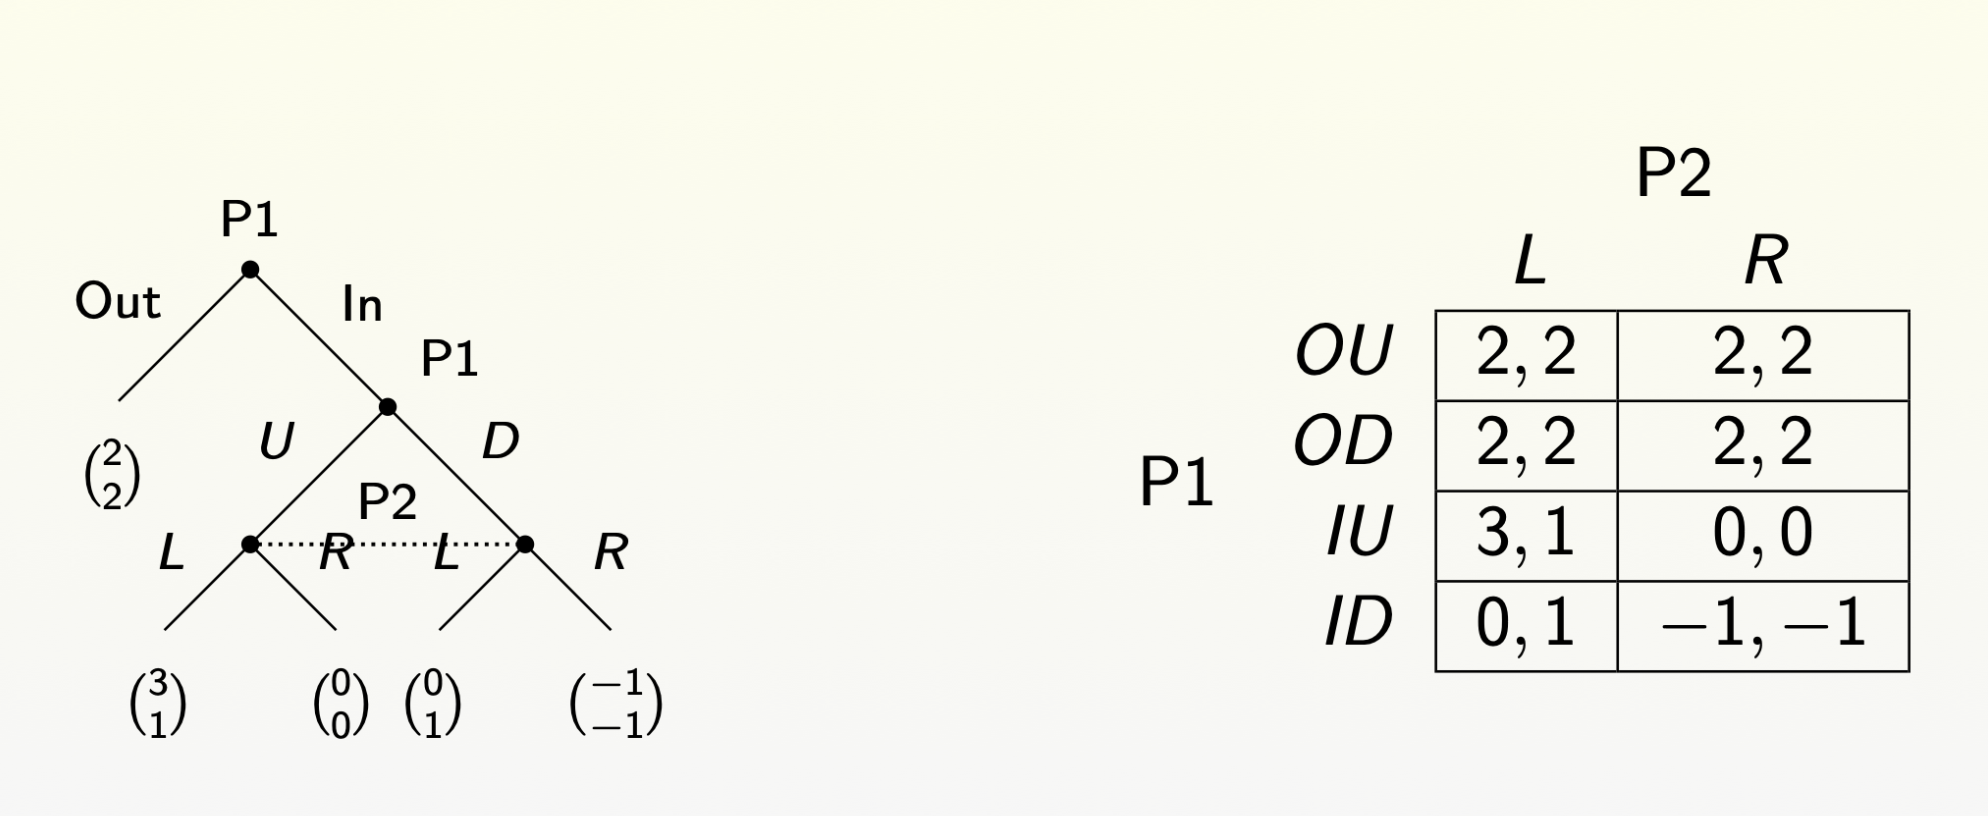
\includegraphics[scale=0.2]{BS.png}
    \caption{Example}
    \label{}
\end{figure}
In this example, a mixed strategy of the P1 can be represented by a probability distribution over $\{OU,OD,IU,ID\}$. To replicate mixed strategy, we can use \textbf{behavioral strategy} that an agent's (probabilistic) choice at each node is independent of his/her choices at other nodes.
\begin{example}
    \begin{enumerate}
        \item Mixed Strategy: $OU$ with probability $\frac{1}{2}$ and $ID$ with probability $\frac{1}{2}$.
        \item Behavioral Strategy: play $O$ and $I$ with prob $\frac{1}{2}$ each at $h = \emptyset$;
        and then $D$ with prob $1$ at history $h = I$.
    \end{enumerate}
\end{example}

\begin{definition}[Behavioral Strategy]
    %\normalfont
    A \textbf{behavioral strategy} for player $i$ is a function that maps histories $h \in H_i$ into probability distributions over $A_i(h)$,
    $$\sigma_i(h)\in\Delta(A_i(h))$$
\end{definition}

A profile of behavioral strategies, $\sigma=\{\sigma_i:i\in N\}$, includes a probability distribution over $Z$. So does a profile of mixed strategies. Then $u_i(\sigma)$ is the expected payoff.

\begin{theorem}[Outcome Equivalent]
    Behavioral and mixed strategies are ``outcome equivalent'' in games of \textbf{perfect recall}.
\end{theorem}
Without perfect recall, behavioral and mixed strategies are not equivalent.


\subsection{Subgame Perfect Equilibrium}
\begin{definition}
    %\normalfont
    A strategy profile $\sigma^*$ is a \textbf{Nash equilibrium} if, for all $i$,
    \begin{enumerate}
        \item $\sigma_i^*$ is the best response to beliefs $\mu_i$,
        \item $\mu_i$ coincides with $\sigma_{-i}^*$.
    \end{enumerate}
\end{definition}
When $s$ is a pure-strategy Nash eq. $h(s)$ is the equilibrium path of $s$.

\begin{definition}
%\normalfont
For games of perfect and complete information, a subgame of an extensive-form game $G=\{N,A,H,Z,P,O,o,\succ_{n\in N}\}$ is a game that starts after a given finite history $h \in H$.

Formally, the subgame $\Gamma(h)$ associated with $h=(h_1,...,h_n)\in H$ is $\Gamma(h)=\left(N,A,H_h,P_h,\{u_{i,h}\}_{i\in N}\right)$, where $H_h=\{(a_1,a_2,...):(h_1,...,h_n,a_1,a_2,...)\in H\}$. $P_h(h')=P(hh')$ for all non-terminal $h'\in H_h$, and $u_{i,h}=u_i(hh')$ for any terminal $h'\in H$.

The game as a whole is a subgame. All other subgames are called proper subgames.
\end{definition}

For a strategy profile $\sigma$:
- $\sigma|h$ denotes the continuation strategy profile in the subgame beginning at $h$
- $z(\sigma|h)$ denotes the terminal node reached by $\sigma$ beginning from $h$
- $u_i(\sigma|h)$ denotes the continuation payoffs

A behavioral strategy $\sigma_i$ of $i$ in $\Gamma$ defines a behavioral strategy $\sigma_i(\cdot|h)$ of $\Gamma(h)$ by $\sigma_i(h'|h)=\sigma_i(hh')$.

\begin{definition}[Subgame Perfect Equilibrium]
    %\normalfont
    A \textbf{subgame perfect equilibrium}[SPNE/SPE] of $\Gamma$ is a strategy profile $\sigma^*$ such that for every subgame $\Gamma(h)$, the continuation strategy profile $\sigma^*|h$ is a Nash equilibrium of $\Gamma(h)$, i.e.,
    $$u_i(\sigma^*|h) \geq u_i((\sigma_i',\sigma_{-i}^*)|h)$$
    for every strategy $\sigma_i'$ and every player $i$.
\end{definition}

Over time $t=1,...,T$, the set of actions is $A^T$.

\begin{lemma}
    $\sigma^*$ is a SPNE \underline{iff} its restriction $\sigma^*(\cdot|h)$ is SPNE of $\Gamma(h)$, for all subgames $\Gamma(h)$.
\end{lemma}

\begin{theorem}[Zermelo's Theorem]
Any finite perfect (and complete) information game has at least one pure-strategy SPE which can be found by backward induction. Furthermore, any such game has a unique SPE if payoffs are generic (i.e., for any pair of terminal nodes $z \neq z'$ implies $u_i(z) \neq u_i(z')$ for all $i$).
\end{theorem}

\subsection{One-Stage Deviation for Finite and Infinite Horizon Games}
\begin{definition}[Finite Horizon]
    %\normalfont
    An extensive-form game has a \textbf{finite horizon} if there is a bound on the length of any history in $Z$.
\end{definition}

In finite horizon games, SPNE can be found through backward induction. For infinite horizon games, we cannot use backward induction directly. Instead, we can think of backward induction as constructing a strategy that is unimprovable by one-stage deviations.

\begin{definition}[One-Stage Deviation]
Let $\sigma_i, \sigma_i'$ be two distinct strategies for player $i$. Let $h$ be a node at which $i$ moves. Let $d_h(\sigma_i,\sigma_i')$ be the strategy that coincides with $\sigma_i$ at all nodes except $h$, where it is determined by $\sigma_i'$, i.e.,
$$d_h(\sigma_i,\sigma_i')(h') = \begin{cases}
\sigma_i(h') & \text{if } h' \neq h\\
\sigma_i'(h') & \text{if } h' = h
\end{cases}$$
Such a strategy is called a one-stage deviation (at $h$).
\end{definition}

\begin{definition}[Unimprovable Strategy]
Fix a strategy profile $\sigma$. A strategy $\sigma_i$ is \textbf{unimprovable by one-stage deviation} if for every $\sigma_i'$ and every $h$ at which $i$ moves:
$$u_i(\sigma|h) \geq u_i((d_h(\sigma_i,\sigma_i'),\sigma_{-i})|h)$$
\end{definition}

\begin{proposition}[One-Stage Deviation Principle for Finite Games]
In any finite perfect and complete information game, any strategy profile that is unimprovable by one-stage deviations is a SPE (and the converse holds).
\end{proposition}

\begin{proof}
The converse is obvious. For the forward direction, suppose $\sigma$ is unimprovable by one-stage deviations but not SPE. Then there exists a subgame $\Gamma(h)$ where some player $i$ has a profitable deviation $\sigma_i'$. Consider the last node $h'$ where $\sigma_i$ and $\sigma_i'$ differ. Then $d_{h'}(\sigma_i,\sigma_i')$ is a profitable one-stage deviation at $h'$, contradicting unimprovability.
\end{proof}

To extend this principle to infinite horizon games, we need an additional condition:

\begin{definition}[Continuous At Infinity]
A perfect and complete information game is \textbf{continuous at infinity} if for every strategy profile $\sigma$, player $i$, history $h$, pair of strategies $\sigma_i,\sigma_i'$, and $\epsilon>0$, there exists an integer $t$ such that the strategy $\tilde{\sigma}_i$ defined by:
$$\tilde{\sigma}_i(h') = \begin{cases}
\sigma_i(h') & \text{if $h'$ is no more than $t$ moves past $h$}\\
\sigma_i'(h') & \text{otherwise}
\end{cases}$$
earns a continuation payoff within $\epsilon$ of $\sigma_i$ in the subgame beginning at $h$.
\end{definition}

\begin{remark}
\begin{itemize}
\item A finite game is continuous at infinity
\item A game with discounting and bounded payoffs is continuous at infinity
\end{itemize}
\end{remark}

\begin{proposition}[One-Stage Deviation Principle]
In any perfect and complete information game that is continuous at infinity, a strategy profile that is unimprovable by one-stage deviations is a subgame perfect Nash equilibrium (and the converse holds).
\end{proposition}

This principle provides the foundation for recursive dynamic programming approaches.

\begin{definition}[Discounted Utility]
%\normalfont
We focus on additively separable models with a sub-utility $u:A \rightarrow \mathbb{R}$ that is the same for each $t$. We model a \textbf{discounted utility} by assuming a discount factor $\delta\in[0,1)$:
\begin{equation}
    \begin{aligned}
        v(a_1,...)=(1-\delta)\sum_{t=1}^\infty \delta^{t-1}u(a_t)
    \end{aligned}
    \nonumber
\end{equation}
\end{definition}

Can think of $\delta$ as the probability that the game will go on for another period, and $1-\delta$ the prob that the game will end.

"Ending" events are independent: A geometric distribution.

The probability that the game ends at time $t$ is $(1 - \delta)\delta^{t-1}$ and $\sum(1-\delta)\delta^t u(a_t)$ becomes expected utility.

\begin{proposition}
    $v(a_1,...)=(1-\delta)\sum_{t=1}^\infty \delta^{t-1}u(a_t)$ is continuous at infinity.
\end{proposition}

\section{Repeated Games}
Let $G_0=\left(N,\{A_i:i\in N\},\{u_i:i\in N\}\right)$ be a normal-form stage game, where $N$ is the set of players, $A_i$ is player $i$'s finite action set, and $u_i$ is player $i$'s payoff function. Let $A=\Pi_{i\in N}A_i$ be the set of action profiles. We only consider games in which $A$ is compact and each $u_i$ is continuous.

Let $T$ be the number of periods (or repetitions) of the repeated game. $T$ can be either finite or infinite.

\begin{definition}[Repeated Game]
    %\normalfont
    A $T$-repeated, $\delta$-discounted game of $G_0$ is an extensive form game $\Gamma=\left(N,A,H,P,\{v_i\}_{i\in N},\delta\right)$, where:
    \begin{enumerate}
        \item $P(h)=N$ for all $h\in H/Z$ (simultaneous moves)
        \item The set of histories $H$ has terminal histories $Z=A^T$
        \item For any sequence of action profiles $\{a(t)\}_{t=1}^T$, player $i$'s payoff is:
        \begin{equation}
            \begin{aligned}
                v_i((a(t))_{t=1}^T)=\left\{\begin{matrix}
                    (1-\delta)\sum_{t=1}^\infty \delta^{t-1}u_i(a(t)),&\delta\in(0,1)\\
                    \sum_{t=1}^T u_i(a(t)),&\delta=1
                \end{matrix}\right.
            \end{aligned}
            \nonumber
        \end{equation}
    \end{enumerate}
\end{definition}

For mixed strategies, let $\alpha_i \in \Delta(A_i)$ denote a mixed action for player $i$. We abuse notation and write $u_i(\alpha)$ for the expected payoff under mixed strategy profile $\alpha$.

\subsection{Nash Reversion Folk Theorem}
\begin{proposition}[Stage-Game NE as SPE]
    If $\{\alpha(t)\}_{t=1}^T$ is a sequence of stage-game Nash equilibria, then playing $\alpha(t)$ at period $t$ regardless of history is a subgame perfect equilibrium of the repeated game (whether finite or infinite).
\end{proposition}

\begin{proposition}[SPE$\Leftrightarrow$No Profitable One-Stage Deviation (Infinite Horizon)]
    Let $\Gamma$ be a discounted, infinitely repeated game. A strategy profile constitutes a subgame perfect equilibrium (SPE) of $\Gamma$ if and only if no player can benefit from deviating in a single stage while conforming to the original strategy in all other stages.
\end{proposition}

\begin{theorem}[Nash Reversion Folk Theorem (Friedman, 1971)]
Let $\alpha^*$ be a Nash equilibrium of the stage game, and let $a \in A$ be a feasible action profile such that $u_i(a) > u_i(\alpha^*)$ for all $i \in N$. Then there exists $\underline{\delta} < 1$ such that for all $\delta \in (\underline{\delta},1)$, there exists a subgame perfect equilibrium of the infinitely repeated game with discount factor $\delta$ where $a$ is played in every period on the equilibrium path.
\end{theorem}

The proof is constructive: Consider the strategy profile where players play $a$ on the equilibrium path and revert to playing the Nash equilibrium $\alpha^*$ forever if any player deviates. For sufficiently patient players (high $\delta$), the long-term loss from punishment outweighs the short-term gain from deviation, making cooperation sustainable as a subgame perfect equilibrium.

\subsection{General Folk Theorem}
\begin{definition}[Minmax Value]
    Let $M_{-j}$ be a profile of mixed strategies in the stage game for all players except $j$ such that
    $$M_{-j} \in \argmin_{\alpha_{-j}} \max_{\alpha_j} u_j(\alpha_j,\alpha_{-j})$$
    Player $j$'s minmax value is:
    $$\underline{v}_j = \max_{\alpha_j} u_j(\alpha_j,M_{-j})$$
\end{definition}

A payoff profile $v=(v_1,\ldots,v_n)$ is feasible if $v=u(a)$ for some $a \in A$.

\begin{theorem}[General Folk Theorem (Fudenberg-Maskin, 1986)]
    Suppose a "full dimensionality condition" is satisfied. For any feasible payoff profile $v$ such that $v_i > \underline{v}_i$ for all $i$, and any $\epsilon > 0$, there exists $\underline{\delta} < 1$ such that for all $\delta \in (\underline{\delta},1)$, there exists a subgame perfect equilibrium where the long-run payoff profile on the equilibrium path lies in the $\epsilon$-neighborhood of $v$.
\end{theorem}

\begin{remark}
    If randomization is observable, we can implement $v$ exactly in every period without the $\epsilon$ approximation. The proof is constructive: If a player deviates, that player is minmaxed for $T$ periods before returning to cooperation. A key difficulty is that minmaxing player $i$ may require player $j$ to receive less than their minmax payoff, necessitating later compensation. The full dimensionality condition ensures such compensation is feasible.
\end{remark}

This theorem shows the multiplicity of equilibria, making equilibrium selection an important open question studied through approaches like evolutionary arguments (Fudenberg-Maskin) and experiments (Dal Bo-Frechette).

\subsection{Folk Theorem in Finite Horizon}

\section{Dynamic Competition}
\begin{enumerate}
    \item Detection lags incurs more competition.
    \item Firm asymmetry leads to more competition.
    \item Multi-market compact may increase the collusion.
    \item Larger number of competitors / Longer horizon increases the competition.
\end{enumerate}


Suppose there are two firms with marginal cost $c$ selling homogeneous products. The demand follows
\begin{equation}
    \begin{aligned}
        D_i(p_i,p_j)=\left\{\begin{matrix}
            D_i(p_i),& p_i<p_j,\\
            \frac{1}{2}D_i(p_i),& p_i=p_j,\\
            0,& p_i>p_j
        \end{matrix}\right.
    \end{aligned}
    \nonumber
\end{equation}
Suppose there is a finite time $T$. The payoff of firm $i$ is
\begin{equation}
    \begin{aligned}
        \sum_{t=1}^T\delta^{t-1} \Pi^i(p_{it},p_{jt})
    \end{aligned}
    \nonumber
\end{equation}
($\delta$ can be written as $\delta=\frac{1}{1+r}$).

When deciding $p_{it}$, the firm $i$ knows history until $t-1$.

$T=1$ (only one period): it is exactly the static case. $p_1=p_2=c$.

For any finite $T$ (finite periods): Since we must have $p_{1T}=p_{2T}=c$ in the period T, we must have $p_{1t}=p_{2t}=c$ in any period.

\subsection{Infinite Periods}
$p_{1t}=p_{2t}=c$ is still an equilibrium.

Another equilibrium can be achieved by the strategy: Collude at monopoly price $p^M:=\argmax_{p}(p-c)D(p)$ (denote the total profit in each period as $\Pi^M:=\max_{p}(p-c)D(p)$) and move to $p=c$ if the competitor deviates. The existence of this equilibrium requires
\begin{equation}
    \begin{aligned}
        \sum_{t=1}^\infty\delta^{t-1}\frac{\Pi^M}{2}\geq \Pi^M
        \Leftrightarrow \delta\geq \frac{1}{2}
    \end{aligned}
    \nonumber
\end{equation}
(Folk Theorem)

\paragraph*{$N$ Competitors}
In the case of $N$ competitors, the condition becomes
\begin{equation}
    \begin{aligned}
        \sum_{t=1}^\infty\delta^{t-1}\frac{\Pi^M}{N}\geq \Pi^M
        \Leftrightarrow \delta\geq 1-\frac{1}{N}
    \end{aligned}
    \nonumber
\end{equation}

\paragraph*{Detection Lags}
The deviation is not detected at once, suppose after two periods. Then the condition becomes
\begin{equation}
    \begin{aligned}
        \sum_{t=1}^\infty\delta^{t-1}\frac{\Pi^M}{2}\geq (1+\delta)\Pi^M
        \Leftrightarrow \delta\geq \frac{1}{\sqrt{2}}
    \end{aligned}
    \nonumber
\end{equation}

\paragraph*{Barriers to Entry}

\paragraph*{Differentiation} Higher differentiation makes collusion less likely, as it decreases the punishment.

\paragraph*{Fluctuations in Demand}
When demand is high, firms have a higher temptation to deviate $\Rightarrow$ Price Wars during booms.

\paragraph*{Secrete Price Cuts with Demand Fluctuations} Suppose the prices are not observed but the demand fluctuates. Given a decrease in sales, you do not know whether it is incurred by the competitor's deviation or the fluctuation of the demand. Firms give punishment in some degree $\Rightarrow$ Price wars during recessions.

\paragraph*{Cost Asymmetries}

\paragraph*{Multi-Market Contract}
Suppose there are two markets: Market A meets every period and Market B meet every two periods.

As we know the collusion occurs in A if $\delta\geq \frac{1}{2}$ and in B if $\delta\geq \frac{1}{\sqrt{2}}$, if $A$ and $B$ are separated.

If we consider these two markets together, the condition is
\begin{equation}
    \begin{aligned}
        \sum_{t=1}^\infty\delta^{t-1}\frac{\Pi^M}{2}+\sum_{t=1}^\infty\delta^{2t-2}\frac{\Pi^M}{2}\geq 2\Pi^M
    \end{aligned}
    \nonumber
\end{equation}
Therefore, there exists $\delta\in \left[\frac{1}{2},\frac{1}{\sqrt{2}}\right]$ that can make collusion in both markets.


\subsection{Empirical Analysis}
Suppose the demand in time $t$ at market $s$ is given by
\begin{equation}
    \begin{aligned}
        P_{ts}=f\left(q_{1ts}+q_{2ts},Z_{ts}\right)
    \end{aligned}
    \nonumber
\end{equation}
where $q$'s are quantities and $Z$ is IV.

The cost of production is given by
\begin{equation}
    \begin{aligned}
        C_{its}=F_{its}+C^{VC}\left(q_{its},w_{ts}\right)
    \end{aligned}
    \nonumber
\end{equation}
where $F_{its}$ is the fixed cost, $C^{VC}(\cdot)$ is the variance cost, and $w_{ts}$ are prices of inputs.
\begin{enumerate}
    \item In perfect competition, $P_{ts}=MC_{its}$.
    \item In perfect collusion, $(q_{1ts},q_{2ts})=\argmax P_{ts}Q_{ts}-C_{1ts}-C_{2ts}$, where $Q_{ts}=q_{1ts}+q_{2ts}$. The F.O.C. is
    \begin{equation}
        \begin{aligned}
            P_{ts}+Q_{ts}\frac{\partial P_{ts}}{\partial q_{1ts}}-MC_{its}=0\\
            P_{ts}=MC_{its}-Q_{ts}\frac{\partial P_{ts}}{\partial q_{1ts}}
        \end{aligned}
        \nonumber
    \end{equation}
    \item Cournot competition: $P_{ts}=MC_{its}-\frac{1}{2}Q_{ts}\frac{\partial P_{ts}}{\partial q_{1ts}}$.
\end{enumerate}

Then, testing the perfect competition or collusion, can be given by estimating the $\theta$:
\begin{equation}
    \begin{aligned}
        P_{ts}=MC_{its}-\theta Q_{ts}\frac{\partial P_{ts}}{\partial q_{1ts}}
    \end{aligned}
    \nonumber
\end{equation}
\begin{enumerate}
    \item Perfect competition: $H_0: \theta=0$
    \item Perfect collusion: $H_0: \theta=1$
    \item Cournot competition: $H_0: \theta=\frac{1}{2}$
\end{enumerate}

\subsection{Market Continue with Probability $x$}
Suppose the market continues with probability $x$. The condition becomes
\begin{equation}
    \begin{aligned}
        \sum_{t=1}^\infty (x\delta)^{t-1}\frac{\Pi^M}{2}\geq \Pi^M
        \Leftrightarrow \delta\geq \frac{1}{2x}
    \end{aligned}
    \nonumber
\end{equation}











\chapter{Signaling}
\section{Signaling Game}
\subsection{Canonical Game}
\begin{definition}[Canonical Game]
    %\normalfont
    \begin{enumerate}
        \item There are two players: $\mathbf{S}$ (sender) and $\mathbf{R}$ (receiver).
        \item $\mathbf{S}$ holds more information than $\mathbf{R}$: the value of some random variable $t$ with support $\mathcal{T}$. (We say that $t$ is the \textbf{type} of $\mathbf{S}$)
        \item Prior belief of $\mathbf{R}$ concerning $t$ are given by a probability distribution $\rho$ over $\mathcal{T}$ (common knowledge)
        \item $\mathbf{S}$ sends a \textbf{signal $s\in \mathcal{S}$} to $\mathbf{R}$ drawn from a signal set $\mathcal{S}$.
        \item $\mathbf{R}$ receives this signal, and then takes an \textbf{action} $a\in \mathcal{A}$ drawn from a set $\mathcal{A}$ (which could depend on the signal $s$ that is sent).
        \item $\mathbf{S}$'s payoff is given by a function $u: \mathcal{T}\times \mathcal{S} \times \mathcal{A} \rightarrow \mathbb{R}$ and $\mathbf{R}$'s payoff is given by a function $v: \mathcal{T}\times \mathcal{S} \times \mathcal{A} \rightarrow \mathbb{R}$.
    \end{enumerate}
\end{definition}

\subsection{Nash Equilibrium}
\begin{definition}[Strategy]
    %\normalfont
    A \textbf{behavior strategy} for $\mathbf{S}$ is given by a function $\sigma: \mathcal{T}\times\mathcal{S} \rightarrow [0,1]$ such that $\sum_s \sigma(t,s)$ for each $t$.\\
    A \textbf{behavior strategy} for $\mathbf{R}$ is given by a function $\alpha: \mathcal{S}\times\mathcal{A} \rightarrow [0,1]$ such that $\sum_a \alpha(s,a)$ for each $t$.
\end{definition}

\begin{definition}[Nash Equilibrium]
    %\normalfont
    Behavior strategies $\alpha$ and $\sigma$ form a \textbf{Nash equilibrium} if and only if
    \begin{enumerate}
        \item For all $t\in \mathcal{T}$,
        \begin{center}
            $\sigma(t,s)>0$ implies $\sum_a \alpha(s,a)u(t,s,a) = \max_{s'\in \mathcal{S}}\left(\sum_a \alpha(s',a)u(t,s',a)\right)$
        \end{center}
        \item For each $s\in \mathcal{S}$ such that $\sum_{t}\sigma(t,s)\rho(t)>0$,
        \begin{center}
            $\alpha(s,a)>0$ implies $\sum_{t}\mu(t;s)v(t,s,a) = \max_{a'}\sum_{t}\mu(t;s)v(t,s,a')$
        \end{center}
        where $\mu(t;s)$ is the $\mathbb{R}$'s posterior belief about $t$ given $s$, $\mu(t;s)=\frac{\sigma(t,s)\rho(t)}{\sum_{t'}\sigma(t',s)\rho(t')}$ if $\sum_t\sigma(t,s)\rho(t)>0$ and $\mu(t;s)=0$ otherwise.
    \end{enumerate}
\end{definition}

\begin{definition}[Separating \& Pooling Equilibrium]
    %\normalfont
    An equilibrium $(\sigma,\alpha)$ is called a \textbf{separating} equilibrium if each type $t$ sends different signals; i.e., the set $\mathcal{S}$ can be partitioned into (disjoint) sets $\{\mathcal{S}_t; t\in \mathcal{S}\}$ such that $\sigma(t, \mathcal{S}_t) = 1$. An equilibrium $(\sigma,\alpha)$ is called a \textbf{pooling} equilibrium if there is a single signal $s^*$ that is sent by all types; i.e., $\sigma(t, s^*) = 1$ for all $t\in \mathcal{T}$.
\end{definition}


\subsection{Single-crossing}

\subsubsection{Situation over real line}
Consider the situation that $\mathcal{T},\mathcal{S},\mathcal{A}\subseteq \mathbb{R}$ and $\geq$ is the usual "greater than or equal to" relationship.

\begin{enumerate}
    \item We let $\Delta \mathcal{A}$ denote the set of probability distributions on $\mathcal{A}$.
    \item For each $s\in \mathcal{S}$ and $\mathcal{T}'\subseteq \mathcal{T}$, we let $\Delta\mathcal{A}(s,T')$ be the set of mixed strategies that are the best responses by $\mathbf{R}$ to $s\in \mathcal{S}$ for some probability distribution with support $\mathcal{T}'$.
    \item For $\alpha\in \Delta\mathcal{A}$, we write $u(t,s,\alpha)\triangleq \sum_{a\in \mathcal{A}}u(t,s,a)\alpha(a)$.
\end{enumerate}

\begin{definition}[Single-crossing]
    %\normalfont
    The data of the game are said to satisfy the \textbf{single-crossing property} if the following holds: If $t\in \mathcal{T}$, $(s,\alpha)\in \mathcal{S}\times \Delta\mathcal{A}$ and $(s',\alpha')\in \mathcal{S}\times \Delta\mathcal{A}$ are such that $\alpha\in \Delta\mathcal{A}(s,\mathcal{T})$, $\alpha'\in \Delta\mathcal{A}(s',\mathcal{T})$, $s>s'$ and $u(t,s,\alpha)\geq u(t,s',\alpha')$, then for all $t'\in T$ such that $t'>t$, $u(t',s,\alpha)\geq u(t',s',\alpha')$.
\end{definition}

\section{Adverse Selection}
Consider a labor market that has many identical firms. In competitive equilibrium, firms' profits are $0$. Firms are price (wage) takers, risk-neutral, and CRS. There are continuum of workers with productivity levels $\theta\in\left[\underline{\theta},\overline{\theta}\right]$ (Assume workers work if it is indifferent for them between employment and non-employment).
\begin{enumerate}
    \item $\theta\sim F$, $F(\cdot)$ is a c.d.f. over $\left[\underline{\theta},\overline{\theta}\right]$.
    \item $N$ is the total mass of workers.
    \item Type $\theta$ worker has a reservation utility $r(\theta)$.
\end{enumerate}

\begin{enumerate}[$\circ$]
    \item Suppose the competitive equilibrium wages are $\theta=w^*(\theta)$.
    \item An allocation is denoted by $I:\left[\underline{\theta},\overline{\theta}\right] \rightarrow \{0,1\}$, where $I(\theta)=0$ denotes $\theta$ is unemployed and $I(\theta)=1$ denotes $\theta$ is employed.
    \item Aggregate welfare = sum of utilities of all participants
    \begin{equation}
        \begin{aligned}
            =N\int_{\underline{\theta}}^{\overline{\theta}} \left[I(\theta)\times\theta+[1-I(\theta)]r(\theta)\right]dF(\theta)
        \end{aligned}
        \nonumber
    \end{equation}
    Then we have the optimal allocation satisfies
    \begin{equation}
        \begin{aligned}
            I^*(\theta)\left\{\begin{matrix}
                =1,&\theta>r(\theta)\\
                \in\{0,1\}&\theta=r(\theta)\\
                =0,&\theta<r(\theta)
            \end{matrix}\right.
        \end{aligned}
        \nonumber
    \end{equation}
\end{enumerate}
In the asymmetric information case,
\begin{definition}
%\normalfont
$w$ is CE wage if $w=\mathbb{E}[\theta|r(\theta)\leq w]$.
\end{definition}

\subsection{Adverse Selection}
\begin{assumption}
    \begin{enumerate}[({A}1).]
        \item $r$ is strictly increasing in $\theta$.
        \item $F(\cdot)$ has a strictly positive density, $F(\theta)>0, \forall \theta\in \left[\underline{\theta},\overline{\theta}\right]$.
        \item $r(\theta)\leq\theta$ (outside option is worse than productivity, i.e., full employment is optimal).
    \end{enumerate}
\end{assumption}

\begin{lemma}
    Under A1-A3, $\Phi(w):=\mathbb{E}[\theta|r(\theta)\leq w]$ is well-defined, continuous, and non-decreasing.
\end{lemma}

Hence, there exists underemployment, which makes $1^{st}$ welfare theorem fails. There may exist multiple CEs, where the one with the highest wage Pareto dominates others.

\begin{example}
    Suppose $\theta\in[0,2]$, $F(\theta)=\frac{\theta}{2}$, $f(\theta)=\frac{1}{2}$, $r(\theta)=\alpha\theta,\alpha\in(0,1)$.
    \begin{equation}
        \begin{aligned}
            \mathbb{E}[\theta|r(\theta)\leq w]=\mathbb{E}\left[\theta|\theta \leq \frac{w}{\alpha}\right]=\left\{\begin{matrix}
                1,&w\geq 2\alpha\\
                \frac{1}{F\left(\frac{w}{\alpha}\right)}\int_0^{\frac{w}{\alpha}}\theta f(\theta)d\theta=\frac{w}{2\alpha},&w\leq 2\alpha
            \end{matrix}\right.
        \end{aligned}
        \nonumber
    \end{equation}
    CEs are given by $\mathbb{E}[\theta|r(\theta)\leq w]=w$. $w^*=0$ is always CE and $w^*=1$ is CE if $\alpha\leq\frac{1}{2}$.
\end{example}

\subsection{Game Theoretical Approach}
\begin{enumerate}
    \item Suppose there are two firms setting wages simultaneously.
    \item Workers observe the wages in stage 1 and make an employment decision.
\end{enumerate}
Let $W^*$ be the set of CE wages and $w^*:=\max W^*$.
\begin{lemma}\label{lemma:ad_l2}
    $\forall w'\in\left(w^*,\overline{\theta}\right]$: $\mathbb{E}[\theta|r(\theta)\leq w']<w'$.
\end{lemma}
\begin{proof}
    Suppose by the contradiction that $\exists w'\in \left(w^*,\overline{\theta}\right]$ s.t. $\mathbb{E}[\theta|r(\theta)\leq w']\geq w'$. Since $\mathbb{E}[\theta|r(\theta)\leq \overline{\theta}]<\overline{\theta}$, there must exist a $w''\in [w',\overline{\theta})$ s.t. $\mathbb{E}[\theta|r(\theta)\leq w'']=w''$ by intermediate value theorem, which contradicts to the definition of $w^*$.
\end{proof}

\begin{proposition}
    \begin{enumerate}[(i).]
        \item If $w^*>r(\underline{\theta})$ and $\exists \epsilon>0$ s.t. $\mathbb{E}[\theta|r(\theta)\leq w']>w',\forall w'\in \left(w^*-\epsilon,w^*\right)$. Then, there is a unique SPE where both firms set wage $=w^*$.
        \item If $w^*=r(\underline{\theta})$ (complete market shutdown at $w^*$), there are multiple SPE that all give the same outcome as complete market shutdown where both firms set wage $=w^*$.
    \end{enumerate}
\end{proposition}
\begin{proof}
    \begin{lemma}\label{lemma:p1}
        In all SPE, firms make zero profits.
    \end{lemma}
    \begin{proof}
        Suppose not, i.e., at least one firm makes strictly positive profits. Then, the total profits of firms $1\&2$, $$\Pi=M(\bar{w})\left[\mathbb{E}[\theta|r(\theta)\leq\bar{w}]-\bar{w}\right]>0$$
        where $\bar{w}$ is the max wage set by the two firms and $M(\bar{w})$ is the mass of workers willing to work at $\bar{w}$. At least one firm, $i$, makes profit $\leq\frac{\Pi}{2}$. Then, $i$'s profits from setting $\bar{w}+\delta$, with $\delta \rightarrow 0^+$, is higher:
        \begin{equation}
            \begin{aligned}
                &M(\bar{w}+\delta)\left[\mathbb{E}[\theta|r(\theta)\leq\bar{w}+\delta]-\bar{w}-+\delta\right]\\
                \geq &M(\bar{w})\left[\mathbb{E}[\theta|r(\theta)\leq\bar{w}+\delta]-\bar{w}-+\delta\right] \rightarrow \Pi \textnormal{ as }\delta \rightarrow 0
            \end{aligned}
            \nonumber
        \end{equation}
        Hence, the $i$ has incentive to deviate.
    \end{proof}
    \begin{lemma}\label{lemma:p2}
        In all SPE, firm $i$ sets $w_i\leq w^*, i\in\{1,2\}$.
    \end{lemma}
    \begin{proof}
        Directly given by Lemma \ref{lemma:ad_l2} and Lemma \ref{lemma:p1}.
    \end{proof}
    \begin{enumerate}[(i):]
        \item In SPE, no firm $i$ sets $w_i<w^*$: suppose $w_i<w^*$ and let $j\neq i$, take any $w'_j$ s.t. $w'_j\in\left(w_i,w^*\right)$ and $w'_j>w^*-\epsilon$. Then, $j$ gets profit: $M(w'_j)\left[\mathbb{E}[\theta|r(\theta)\leq w'_j]-w'_j\right]>0$ (by Case (i)'s conditions).
        \item By Lemma \ref{lemma:p2}, both firms set $w_i\leq w^*=r(\underline{\theta})$. Check that $\{(w_1,w_2):w_1,w_2\leq w^*\}$ is SPE wage profiles.
    \end{enumerate}
\end{proof}

\subsection{Planner Intervention}
Planner can't observe the true type $\theta$.

The planner's tools:
\begin{enumerate}
    \item Take over the firms.
    \item $w_e$, employment wage.
    \item $w_u$, unemployment wage.
\end{enumerate}
s.t. budget balanced.

\begin{definition}[Constrained Efficient]
    %\normalfont
    A CE $w$ is \textbf{constrained efficient} if it cannot be Pareto improved upon by an intervention by the planner.
\end{definition}

\begin{proposition}[$w^*:=\max W^*$ is constrained efficient]
    Let $W^*$ be the set of CE wages. $w^*:=\max W^*$ is constrained efficient.
\end{proposition}
\begin{proof}
    Note that both firms are making zero profits by the Lemma \ref{lemma:p1}. Any CE wage $w\neq w^*$ can be Pareto improved by $\{w_e=w^*,w_u=0\}$. Then, we prove $w^*$ can't be Pareto improved.
    \begin{enumerate}
        \item Case 1: if $w^*$ gives full-employment in CE, then $w^*$ is Pareto efficient.
        \item Case 1: suppose $w^*$ doesn't give full-employment in CE.
        
        Consider taking an intervention $w_e\&w_u$. Then, $\{\theta:r(\theta)+w_u\leq w_e\}=[\underline{\theta},\hat{\theta}]$ for some $\hat{\theta}\in[\underline{\theta},\overline{\theta}]$ such that
        \begin{equation}
            \begin{aligned}
                r(\hat{\theta})+w_u=w_e
            \end{aligned}
            \label{con:1}
        \end{equation}
        The budget balanced gives
        \begin{equation}
            \begin{aligned}
                w_e F(\hat{\theta})+w_u (1-F(\hat{\theta}))=\int_{\underline{\theta}}^{\hat{\theta}}\theta d F(\theta)
            \end{aligned}
            \label{con:2}
        \end{equation}
        Plug \eqref{con:1} into \eqref{con:2}:
        \begin{equation}
            \begin{aligned}
                \left\{\begin{matrix}
                    &w_u(\hat{\theta})=\int_{\underline{\theta}}^{\hat{\theta}}\theta d F(\theta)-r(\hat{\theta})F(\hat{\theta})=F(\hat{\theta})\left(\mathbb{E}[\theta|\theta\leq\hat{\theta}]-r(\hat{\theta})\right)\\
                    &w_e(\hat{\theta})=\int_{\underline{\theta}}^{\hat{\theta}}\theta d F(\theta)+r(\hat{\theta})(1-F(\hat{\theta}))
                \end{matrix}\right.
            \end{aligned}
            \nonumber
        \end{equation}
        Let $\theta^*$ be s.t. $r(\theta^*)=w^*$. Because $w^*$ is a CE price, $\mathbb{E}[\theta|\theta\leq\theta^*]=r(\theta^*)=w^*$. So, CE with $w^*$ can be implemented by $w_u(\theta^*)=0$ and $w_e(\theta^*)=w^*$.
        \begin{enumerate}
            \item If $\hat{\theta}<\theta^*$. $\underline{\theta}$ is worse off under the intervention since $w_e(\hat{\theta})<w^*$.
            \item If $\hat{\theta}>\theta^*$. $\overline{\theta}$ is worse off under the intervention since $w_u(\hat{\theta})=F(\hat{\theta})\left(\mathbb{E}[\theta|\theta\leq\hat{\theta}]-r(\hat{\theta})\right)<0$ by the Lemma \ref{lemma:ad_l2}
        \end{enumerate}
    \end{enumerate}
\end{proof}


\subsection{Signaling}\label{sec:signaling}
Suppose the worker $\theta\in[\underline{\theta},\overline{\theta}]$ can properly and costlessly reveal his type to the firms. Then,
\begin{lemma}
    All workers revel their types.
\end{lemma}
\paragraph*{Spence's Job Market Signaling Model} One worker has productivity $\theta\in\{\theta_L,\theta_H\}$ with $P(\theta_H)=\lambda$. The worker signal through his education with cost $e>0$. The education doesn't change his productivity. The payoff of the worker is the wage minus the cost:
\begin{equation}
    \begin{aligned}
        u(w,e|\theta)=w-c(e,\theta)
    \end{aligned}
    \nonumber
\end{equation}
where $c(0,\theta)=0,c_e(e,\theta):=\frac{\partial c(e,\theta)}{\partial e}>0, c_\theta(e,\theta):=\frac{\partial c(e,\theta)}{\partial \theta}<0$, and $c_{e\theta}(e,\theta):=\frac{\partial^2 c(e,\theta)}{\partial e\partial \theta}<0$ (Single-Crossing Property, the difference $c(e,\theta_L)-c(e,\theta_H)$ is increasing in $e$ (i.e., $c_e(e,\theta_L)-c_e(e,\theta_H)>0$), which means if $c(e,\theta_L)$ and $c(e,\theta_H)$ intersect as functions of $e$, they only intersect at one time.)
\begin{enumerate}[]
    \item \underline{Stage 0}: Nature chooses the $\theta\in\{\theta_L,\theta_H\}$ with $P(\theta_H)=\lambda$.
    \item \underline{Stage 1}: The worker learns $\theta$ and chooses $e(\theta)\geq 0$.
    \item \underline{Stage 2}: Firms observe $e(\theta)$. Then, they simultaneously make wage offers $w_1$ and $w_2$.
    \item \underline{Stage 3}: The worker observes $w_1,w_2$ and makes employment decision.
\end{enumerate}
Let $r(\theta_L)$ and $r(\theta_H)=0$. Let $\mu(e)\in[0,1]$ be the probability that in the beginning of stage 2, firms think that the worker is $\theta_H$ type with probability $\mu(e)$ when observing $e$. The corresponding expected productivity (the highest wage) that the firm can pay is
\begin{equation}
    \begin{aligned}
        w(e)=\mu(e)\theta_H+(1-\mu(e))\theta_L
    \end{aligned}
    \nonumber
\end{equation}
In stage 2, both firm will set $w(e)$ (complete competition).

\begin{definition}[Perfect Bayesian Equilibrium]
    %\normalfont
    A PBE is a strategy profile ($e^*(\theta_L)$, $e^*(\theta_H)$, $w^*_1: \mathbb{R}_+ \rightarrow \mathbb{R}$, $w^*_2: \mathbb{R}_+ \rightarrow \mathbb{R}$), and a belief $\mu^*: \mathbb{R} \rightarrow [0,1]$ such that
    \begin{enumerate}
        \item $\forall \theta\in\{\theta_L,\theta_H\}$, the worker strategy optimal given firm strategies.
        \item The belief $\mu^*(e)$ is derived from $\lambda, e^*(\theta_L), e^*(\theta_H)$ via Bayes' rule whenever possibly (on the equilibrium path). Outside the equilibrium path the belief $\mu^*(e)$ is arbitrarily.
        \item Firms offer wages that form a NE of the stage 2 game, where their belief $\mu^*(e)$ about their workers' type. (sequential rationality).
    \end{enumerate}
\end{definition}
We simplify the game by backward induction:
\begin{enumerate}
    \item \underline{Stage 3}: The worker chooses the highest wage off if it is $\geq 0$.
    \item \underline{Stage 2}: After observing $e(\theta)$, firms chooses the wage as the expected productivity in NE,
    \begin{equation}
        \begin{aligned}
            w^*(e)=\mu^*(e)\theta_H+(1-\mu^*(e))\theta_L
        \end{aligned}
        \nonumber
    \end{equation}
    because it is a Bertrend competition.
\end{enumerate}
\paragraph*{Separating Equilibrium}
In separating equilibrium, $e^*(\theta_L)\neq e^*(\theta_H)$.
\begin{lemma}
    In any separating PBE, $w^*(e^*(\theta))=\theta, \forall \theta\in\{\theta_L,\theta_H\}$.
\end{lemma}
\begin{proof}
    By Bayes' rule, after firm observe $e^*(\theta_L)$, $\mu^*(e^*(\theta_L))=0$. Then, $w^*(e^*(\theta_L))=\theta_L$. ($e^*(\theta_H)$ is similar.)
\end{proof}

\begin{lemma}
    In separating PBE, low type always chooses zero education, $\theta^*(\theta_L)=0$.
\end{lemma}
\begin{proof}
    If not, the low type worker always has profitable deviation, $\theta^*(\theta_L)=0$.
\end{proof}

\begin{lemma}
    Define $\underline{e}$ and $\overline{e}$ such that
    \begin{enumerate}
        \item $\theta_L=\theta_H-c(\underline{e},\theta_L)$ (the lowest effort can prevent the low type from mimicking high type) and
        \item $\theta_L=\theta_H-c(\overline{e},\theta_H)$ (the highest effort can prevent the high type from pooling with low type).
    \end{enumerate}
    Then, in all separating PBEs, $e\in \left[\underline{e},\overline{e}\right]$.\\
    Conversely, $\forall \hat{e}\in \left[\underline{e},\overline{e}\right]$, there is a separating PBE where $e^*(\theta_H)=\hat{e}$.
\end{lemma}
These different PBEs are Pareto ranked. High type prefers the PBE with a lower $e$ (the best is the one with $e^*(\theta_H)=\underline{e}$.)

\paragraph*{Pooling PBE}
$e^*(\theta)=e^*,\theta\in\{\theta_L,\theta_H\}$, $\mu^*(e^*)=\lambda$, and $w^*(e^*)=\mathbb{E}[\theta]$.

\begin{lemma}
    Define $e'$ by $\theta_L=\mathbb{E}[\theta]-c(e',\theta_L)$ (the highest effort can prevent the low type from choosing $e=0$ and get $w=\theta_L$.)\\
    Then, for all pooling PBE, $e^*(\theta_L)=e^*(\theta_H)=e^*\in[0,e']$. Conversely, for all $\hat{e}\in [0,e']$, there is a pooling PBE with $e^*=\hat{e}$.
\end{lemma}


\subsection{Cho-Kreps Intuitive Criterion}
\begin{definition}[Equilibrium Dominated Message]
    %\normalfont
    A message is \textbf{equilibrium dominated} for a type if the type must do strictly worse by sending the message than it does in equilibrium (i.e., payoff in eq. is strictly better than maximum payoff from deviating).
\end{definition}

\begin{definition}[Cho-Kreps Intuitive Criterion]
    %\normalfont
    If an information set is off the eq. path and a message is eq. dominated for a type, then beliefs should assign zero probability to the message coming from that type (if possible).
\end{definition}

Fix a PBE $e^*(\theta), \theta\in\{\theta_L,\theta_H\}, \mu^*(\cdot)$ (We know $w_1^*(e)=w_2^*(e)=\mu(e)\theta_H+(1-\mu(e))\theta_L$). Let $u^*(\theta),\theta\in\{\theta_L,\theta_H\}$ be the PBE utility of the type $\theta$ worker.

The criterion requires the (off-path) belief $\mu^*(e):=P(\tilde{\theta}=\theta_H|e)=1-P(\tilde{\theta}=\theta_L|e)$ satisfies $$P(\tilde{\theta}=\theta|e)=0,\forall e,\theta$$ such that
\begin{enumerate}
    \item $u^*(\theta)>\max_{w\in[\underline{\theta},\overline{\theta}]}[w-c(e,\theta)]$
    \item $\exists \theta'$ s.t. $u^*(\theta')\leq \max_{w\in[\underline{\theta},\overline{\theta}]}[w-c(e,\theta')]$ (make sure the sum of beliefs given $e$ is nonzero.)
\end{enumerate}
In this application, the only PBE that survives Intuitive Criterion is the best separating PBE, $e^*(\theta_H)=\underline{e}$ (the lowest effort).



\subsection{Grossman-Perry-Farrell Equilibrium}
For the equilibrium refinement, we can also introduce the Grossman-Perry-Farrell equilibrium based on the perfect sequential equilibrium (grossman1986sequential) and the neologism-proof equilibrium (farrell1993meaning). We formally define the Grossman-Perry-Farrell equilibrium by ruling out the self-signaling sets in Perfect Bayesian Equilibrium (bertomeu2018verifiable,glode2018voluntary).

A binary example is given as follows:
\begin{definition}[Grossman-Perry-Farrell Equilibrium (GPFE)]
	A pure-strategy perfect Bayesian equilibrium $(p^*_L,p^*_H,b^*(\cdot))$ is a ``Grossman-Perry-Farrell equilibrium'' (GPFE) if there does not exist a self-signaling set, which is defined by a set $\chi\subseteq\{L,H\}$ such that there exists a price $p'$ such that
	\begin{equation}
		\begin{aligned}
			\chi=\{j\in\{L,H\}:U(p',\mu_\chi)>U(p_j^*,b^*(p_j^*))\},
		\end{aligned}
		\nonumber
	\end{equation}
	where $\mu_\chi=\frac{q_L\rho_e\mathbf{1}_{L\in\chi}+q_H(1-\rho_e)\mathbf{1}_{H\in\chi}}{\rho_e\mathbf{1}_{L\in\chi}+(1-\rho_e)\mathbf{1}_{H\in\chi}}$ is the average quality of types in $\chi$ based on the relative prior probabilities.
\end{definition}

\begin{note}
    The GPFE is a strong refinement of PBE that may lead to no equilibrium exists.
\end{note}

\chapter{Screening}
\section{Screening Model}
Workers can undertake a contractible/observable task level $t\geq 0$. The utility of a worker is defined by $u(w,t,\theta):=w-c(t,\theta)$, where $c(\cdot,\cdot)$ satisfies the same assumption as in signaling model \ref{sec:signaling}.

The Game follows
\begin{enumerate}[]
    \item \underline{Stage 1}: Two firms simultaneously determine sets of contracts, $(w,t)$.
    \item \underline{Stage 2}: The worker observes all offer contracts and makes employment decision.
    (If indifference, choose lower task contract, favor employment over unemployment. If contracts of firms are indifferent, choose each with probability 1/2.)
\end{enumerate}

The null contract is $(w,t)=(0,0)$. Assume WLOG at stage 1, each firm appears a non-empty set of contracts.

\subsubsection*{Perfect Information}
\begin{proposition}[Perfect Information]
    If firms can observe the worker types, then in SPE firms make zero profit and type $\theta_i$ worker signs $(w^*_i,t^*_i)=(\theta_i,0)$.
\end{proposition}
\begin{proof}
    \begin{claim}
        Firms make zero profits from this contract.
    \end{claim}
    \begin{proof}
        Suppose not,
    \begin{enumerate}[$\circ$]
        \item $w^*_i>\theta_i$ $\Rightarrow$ negative profits, firms benefit from offering null contract.
        \item $w^*_i<\theta_i$ $\Rightarrow$ Let $\Pi$ be the total profits of the firms. Then one of the firms makes profit $\leq \frac{\Pi}{2}$. Then, this firm can benefit from offering $(w^*_i+\Delta,t^*_i)$, where $\Delta \rightarrow 0^+$.
    \end{enumerate}
    \end{proof}
    Then, we prove the firms must choose $(w^*_i,t^*_i)=(\theta_i,0)$. Suppose by the way of contradiction that $t_i^*>0$. Then, one firm can profitably deviate by offering $(w^*_i,0)$.
\end{proof}

\subsubsection*{Asymmetric Information}
\begin{lemma}\label{lemma:zero_profit}
    In any SPE, firms obtain zero profits,
\end{lemma}
\begin{proof}
    Firms must make profits $\geq 0$. Suppose by the way of contradiction that the total profit $\Pi>0$. Let $(w_L,t_L)$ be the contract signed by $\theta_L$ and $(w_H,t_H)$ be the contract signed by $\theta_H$. One firm can profitably deviate by offering $(w_L+\Delta,t_L)$ and $(w_H+\Delta,t_H)$, where $\Delta \in (0,\Pi)$.
\end{proof}

\begin{lemma}
    There is \textbf{no} pooling SPE.
\end{lemma}
\begin{proof}
    Suppose for a contradiction, $\exists$ an SPE where both worker types sign $(w_p=\mathbb{E}[\theta],t_p)$. Suppose one firm offers $(w_p,t_p)$, then another firm can only employ high type workers by offering $(\tilde{w},\tilde{t})$, where $\tilde{w}-c(\tilde{t},\theta_H)>\mathbb{E}[\theta]-c(t_p,\theta_H)$, $\tilde{w}-c(\tilde{t},\theta_L)<\mathbb{E}[\theta]-c(t_p,\theta_L)$, and $\tilde{w}<\theta_H$. (The existence is given by $\frac{\partial^2 c(t,\theta)}{\partial t\partial \theta}<0$.)
\end{proof}

\begin{lemma}
    Let $(w_L,t_L)$ be the contract signed by $\theta_L$ and $(w_H,t_H)$ be the contract signed by $\theta_H$ in separating SPE. Then, $w_L=\theta_L$ and $w_H=\theta_H$.
\end{lemma}
\begin{proof}
    Suppose $w_i>\theta_i,i\in\{L,H\}$, firms benefit from not offering this contract. So, $w_L\leq \theta_L$ and $w_H\leq \theta_H$.
    \begin{enumerate}
        \item \underline{$w_L=\theta_L$:} Suppose $w_L<\theta_L$. Either firm can profitably deviate by setting $(w'_L,t_L)$ such that $w_L<w'_L<\theta_L$. This offer can win all low-type workers and get a positive profit from hiring them. If $w'_L-c(t_L,\theta_H)\geq w_H-c(t_H,\theta_H)$, the offer can also hire high-type workers, which also give positive profit for the firm. Hence, there is a contradiction.
        \item \underline{$w_H=\theta_H$:} Suppose $w_H<\theta_H$, firms get positive profits, which contradicts to the Lemma \ref{lemma:zero_profit}.
    \end{enumerate}
\end{proof}

\begin{lemma}
    $\theta_L$ signs the contract $(\theta_L,0)$ in SPE.
\end{lemma}
\begin{proof}
    Suppose $t_L>0$. One firm can profitably deviate by offering $(\theta_L-\Delta,0)$.
\end{proof}

\begin{proposition}
    In any (pure strategy) SPE, $\theta_L$ signs $(w_L,t_L)=(\theta_L,0)$ and $\theta_H$ signs $(w_H,t_H)=(\theta_H,t_H)$, where $t_H$ solves
    \begin{equation}
        \begin{aligned}
            \theta_H-c(t_H,\theta_L)=\theta_L
        \end{aligned}
        \nonumber
    \end{equation}
\end{proposition}

If $\lambda:=P(\theta_H)$ is high, the pure SPE may not exist (exist $(\tilde{w},\tilde{t})$ can attract both types and make positive profit).

Cross subsidizing deviation by a firm (prices one product above its market value to fund another product), $(\tilde{w},\tilde{t})$ (signed by low type) and $(\tilde{\tilde{w}},\tilde{\tilde{t}})$ (signed by high type), is a profitable deviation if $\lambda$ is large enough.


\chapter{Bargaining}
Bargaining refers to “a process to determine the terms of trade that is not adequately captured by off-the-shelf oligopoly models.” (Loertscher and Marx, 2021).

\section{Axiomatic Complete Information Bargaining}
The axiomatic approach abstracts away from the specifics of the bargaining process, focusing instead on identifying ``reasonable” or ``natural” properties that outcomes should satisfy.

\subsection{Bilateral Negotiations}
Let $X$ denote the \textit{set of possible agreements} and $D$ the \textit{disagreement} outcome.
\begin{example}
    Suppose $X=\{(x_1,x_2):x_1+x_2=1, x_i\geq 0\}$ and $D=(0,0)$.
\end{example}

Each player $i$ has preferences represented by a utility function $u_i$ defined over $X\cup\{D\}$. The set of possible payoffs, denoted by $U$, is defined as:
\begin{equation}
    \begin{aligned}
        U&=\{(v_1,v_2):u_1(x)=v_1, u_2(x)=v_2 \textnormal{ for some } x\in X\},\\
        d&=\left(u_1(D), u_2(D)\right).
    \end{aligned}
    \nonumber
\end{equation}
\begin{definition}[Bargaining Problem]
    A \textbf{bargaining problem} is a pair $(U,d)$ where $U\subseteq \mathbb{R}^2$ and $d\in U$. Typically, we assume:
    \begin{enumerate}
        \item $U$ is a convex and compact set.
        \item There exists some $v\in U$ such that $v>d$ (i.e., $v_i>d_i$ for all $i$).
    \end{enumerate}
\end{definition}
We denote the set of all possible bargaining problems by $B$. A bargaining solution is a function $f:B \rightarrow U$.

\begin{definition}[Axioms]
    We study bargaining solutions $f(\cdot)$ that satisfy the following axioms:
    \begin{enumerate}
        \item \textbf{Axiom 1 (Pareto Efficiency)}: A bargaining solution $f(U,d)$ is \textit{Pareto efficient} if there does not exist a $(v_1, v_2)\in U$ such that $v\geq f(U,d)$ and $v_i>f_i(U,d)$ for some $i$.
        \begin{note}
            Intuition: An inefficient outcome is unlikely, as it leaves room for renegotiation.
        \end{note}
        \item \textbf{Axiom 2 (Symmetry)}: A bargaining solution $f$ is \textit{symmetric} if for any symmetric bargaining problem $(U,d)$ (i.e., $(u_1,u_2)\in U$ if and only if $(u_2,u_1)\in U$, and $d_1=d_2$), we have $f_1(U,d)=f_2(U,d)$.
        \begin{note}
            Intuition: If the players are indistinguishable, the agreement should not favor one over the other. (This axiom can be relaxed to account for bargaining power.)
        \end{note}
        \item \textbf{Axiom 3 (Invariance to Linear Transformations)}: A bargaining solution $f$ is \textit{invariant} if for any bargaining problem $(U, d)$ and all $\alpha_i\in (0, \infty)$, $\beta_i\in \mathbb{R}$ ($i=1,2$), if we consider the transformed bargaining problem $(U',d')$ with
        \begin{equation}
            \begin{aligned}
                U'&=\{(\alpha_1u_1+\beta_1,\alpha_2u_2+\beta_2):(u_1,u_2)\in U\},\\
                d'&=\left(\alpha_1d_1+\beta_1,\alpha_2d_2+\beta_2\right),
            \end{aligned}
            \nonumber
        \end{equation}
        then $f_i(U',d')=\alpha_i f_i(U,d) + \beta_i$ for $i=1,2$.
        \begin{note}
            Intuition: Utility functions are merely one cardinal representation of ordinal preferences. They lack intrinsic cardinal meaning, so monotonic (especially linear) transformations should not affect the outcome.
        \end{note}
        \item \textbf{Axiom 4 (Independence of Irrelevant Alternatives)}: A bargaining solution $f$ is \textit{independent} if for any two bargaining problems $(U,d)$ and $(U',d)$ with $U'\subseteq U$ and $f(U,d)\in U'$, we have $f(U',d)=f(U,d)$.
        \begin{note}
            Intuition: Removing options that were not chosen should not change the outcome. This axiom arguably reflects behavioral assumptions and may require additional justification.
        \end{note}
    \end{enumerate}
\end{definition}

\subsection{Nash Bargaining Solution}
\begin{definition}[Nash Bargaining Solution]
    The Nash (1950) bargaining solution $f_N$ is defined as:
    \begin{equation}
        \begin{aligned}
            f_N(U,d)=\argmax_{u\in U, u\geq d}\ (u_1-d_1)(u_2-d_2)
        \end{aligned}
        \nonumber
    \end{equation}
\end{definition}
Given the assumptions on $(U, d)$, the solution to this optimization problem exists (if $U$ is compact and the objective function is continuous) and is unique (if the objective function is strictly quasi-concave).

\begin{theorem}[Nash, 1950]
    $f_N$ is the unique bargaining solution that satisfies the four axioms.
\end{theorem}

The Nash bargaining solution can be generalized to account for unequal bargaining weights:
\begin{equation}
    \begin{aligned}
        f_\beta(U,d)=\argmax_{u\in U, u\geq d}\ (u_1-d_1)^{\beta}(u_2-d_2)^{1-\beta}
    \end{aligned}
    \nonumber
\end{equation}
This solution is straightforward to compute and can be microfounded using an alternating offers bargaining game, as in Rubinstein (1982). See, for example, Binmore et al. (1986). Essentially, it selects a point on the efficient frontier (above $d$).

The Nash bargaining solution assumes no breakdown in negotiations.

\begin{note}
    \textbf{Weakness:} In Nash bargaining, the disagreement point plays a disproportionately significant role. If the negotiation is over a set of options that dominates $d$, it is unclear why the disagreement point should matter (e.g., Binmore et al. (1986)). This characteristic of Nash bargaining often has a substantial impact in empirical applications.
\end{note}

\subsection{Multiple Simultaneous Negotiations (Nash-in-Nash)}
\begin{enumerate}
    \item Consider a scenario with a finite set of agents $\{1,...,N\}$.
    \item Let $\mathcal{G}$ represent the set of feasible pairs, $ij$, that can potentially form agreements to collaborate.
    \item Denote $p_{ij}$ as the transfer from agent $j$ to agent $i$ if they reach an agreement.
    \item The value to agent $i$ when a set $A\subseteq \mathcal{G}$ of agreements is realized is $\pi_i(A)$. The net payoff to $i$ is $\pi_i(A)+p_i$, where $p_i$ is the total payment received by $i$.
    \begin{note}
        Agreements may generate externalities, but payments themselves do not.
    \end{note}
    \item For $B\subset A\subset \mathcal{G}$, define $\Delta\pi_i(A,B)=\pi_i(A)-\pi_i(A\setminus B)$ as the marginal value of adding the set $B$ of agreements, given that $A\setminus B$ is already realized.
\end{enumerate}

\begin{assumption}[Gains from Trade]
    For all $ij\in \mathcal{G}$, $\Delta\pi_i(\mathcal{G},ij)+\Delta\pi_j(\mathcal{G},ij)>0$.
\end{assumption}

\begin{definition}[Nash-in-Nash Bargaining Solution]
    In the Nash-in-Nash solution, under the gains-from-trade assumption, all agreements are reached. The transfer from $j$ to $i$ is given by:
    \begin{equation}
        \begin{aligned}
            p_{ij}^N=\argmax_{p}\left(\Delta\pi_i(\mathcal{G},ij)+p\right)^{b_i}\left(\Delta\pi_j(\mathcal{G},ij)-p\right)^{b_j}=\frac{b_i\Delta\pi_j(\mathcal{G},ij)-b_j\Delta\pi_i(\mathcal{G},ij)}{b_i+b_j}.
        \end{aligned}
        \nonumber
    \end{equation}
    In other words, the outcome between each pair is the bilateral Nash bargaining solution, given the “equilibrium” conjecture that all other agreements are reached. This represents a Nash equilibrium in Nash bargaining.
\end{definition}

\begin{remark}
    \textbf{Weakness:}
    \begin{enumerate}
        \item Inherits the limitations of the Nash bargaining solution.
        \item Assumes binary agreements.
        \item Considers externalities only over agreements, not lump-sum payments.
        \item Relies on ``passive beliefs'': if the negotiation between $i$ and $j$ breaks down, $i$ negotiates with $k$ as if the agreement between $i$ and $j$ were still in place.
        \item Assumes complete information.
    \end{enumerate}
\end{remark}


\section{Incomplete Information Bargaining}

\subsection{Bilateral Trade with Incomplete Information}

Consider a bilateral trade setting with:
\begin{itemize}
    \item A buyer $B$ with value $v\in[\underline{v},\bar{v}]$ for a good
    \item A seller $S$ with value (or production cost) $c\in[\underline{c},\bar{c}]$
    \item Types are independently distributed
\end{itemize}

By the revelation principle, we can focus on incentive compatible direct mechanisms, which consist of:

\begin{definition}[Direct Mechanism]
    A direct mechanism in bilateral trade is characterized by:
    \begin{enumerate}
        \item An allocation rule $q:[\underline{v},\bar{v}]\times[\underline{c},\bar{c}]\rightarrow[0,1]$ determining the probability of trade
        \item Payment rules $p_j:[\underline{v},\bar{v}]\times[\underline{c},\bar{c}]\rightarrow\mathbb{R}$ determining the payment made by agent $j\in\{B,S\}$
    \end{enumerate}
\end{definition}

\begin{definition}[Mechanism Properties]
    A mechanism $(q,p)$ is:
    \begin{enumerate}
        \item \textbf{Bayesian incentive compatible (BIC)} if truthful reporting is optimal for each agent at the interim stage (knowing only their own type).
        \item \textbf{Interim IR} if each agent receives a non-negative expected payoff at the interim stage.
        \item \textbf{Dominant strategy incentive compatible (DSIC)} if truthful reporting is optimal for each agent, conditional on each profile of the others' types.
        \item \textbf{Ex-post IR} if each agent receives a non-negative payoff ex-post.
        \item \textbf{No-deficit in expectation} if $E[p_B(v,c)+p_S(v,c)]\geq 0$
        \item \textbf{Budget balanced in expectation} if $E[p_B(v,c)+p_S(v,c)]=0$
        \item \textbf{Efficient} if trade occurs whenever $v>c$, and never if $v<c$
    \end{enumerate}
\end{definition}

\begin{remark}
    BIC, Interim IR, and no-deficit seem reasonable conditions which should be satisfied, at a minimum.
\end{remark}


\begin{theorem}[Myerson-Satterthwaite Impossibility Theorem]
    In the bilateral trade setting, if $\underline{v}<\bar{c}$, then there exists no mechanism that is simultaneously efficient, Bayesian incentive compatible (BIC), interim individually rational (IR), and does not run a deficit in expectation.
    
    In other words, whenever agents have the option to walk away and play a Bayes-Nash equilibrium, trade cannot be efficient.
\end{theorem}

\begin{proof}
    Recall the Revenue Equivalence theorem, which states that we can write the payments made by agent $i$ as a function of the allocation rule, plus the surplus that the mechanism leaves to $i$ when they have the least-favorable type ($\underline{v}$ for buyer, $\bar{c}$ for seller).
    
    Consider the following mechanism that implements the efficient allocation rule:
    \begin{itemize}
        \item Trade occurs if and only if $v\geq c$. The buyer pays $p_B=\max\{c,\underline{v}\}$, and the seller receives $-p_S=\min\{v,\bar{c}\}$. Otherwise, no trade occurs and no payments are made.
    \end{itemize}
    
    This mechanism is dominant strategy incentive compatible (DSIC), and therefore a fortiori BIC. Moreover, the payoff of a type $\underline{v}$ buyer and type $\bar{c}$ seller are both zero. Furthermore, $p_B(v,c)+p_S(v,c)\leq 0$ for all $c$, with strict inequality for almost all types.
    
    By revenue equivalence, any other efficient, IR, and BIC mechanism must have weakly lower revenue (strictly lower if either agent's IR constraint does not bind).
\end{proof}






\subsection{k-Double Auction}
The k-double auction, proposed by Chatterjee and Samuelson (1983), provides a non-cooperative foundation for bargaining in bilateral trade:

\begin{itemize}
    \item Buyer submits a sealed bid $b$
    \item Seller submits a sealed offer $s$ 
    \item Trade occurs if and only if $b \geq s$
    \item If trade occurs, payment from buyer to seller is $kb + (1-k)s$
\end{itemize}

Assume that agents play a Bayes-Nash equilibrium and can walk away before the game begins. This corresponds exactly to the Bayesian incentive compatibility (BIC) and Interim individual rationality (IR) constraints for the direct mechanism. Note that the outcome of the k-double auction is budget balanced by construction.

\begin{example}[Special Equilibrium, posted price]
    Here is a special equilibrium in the k-double auction:
    Fix a price $p \in (\underline{c}, \bar{v})$ and consider the following strategies:
    \begin{itemize}
        \item Buyer: Bid $p$ when $v \geq p$, and bid $\underline{c}$ otherwise
        \item Seller: Ask $p$ when $c \leq p$, and ask $\bar{v}$ otherwise
    \end{itemize}
    Since $kp + (1-k)p = p$, this is equivalent to a posted price mechanism (on the equilibrium path).
\end{example}
\begin{note}
    \begin{enumerate}
        \item Fixing one agent's strategy, the specified strategy is optimal for the other agent ex-post (even if they knew the other's type). Therefore this mechanism can be implemented as a dominant strategy incentive compatible (DSIC) direct mechanism.
        \item Any $p \in (\underline{c}, \bar{v})$ will work as this fixed price.
    \end{enumerate}
\end{note}


\begin{theorem}[DSIC Characterization]
    If $\underline{c} \leq \bar{v}$, then any budget-balanced, ex-post individually rational, dominant strategy incentive compatible (DSIC) mechanism that is not Pareto dominated must be a randomization over posted price mechanisms.
\end{theorem}

\begin{proof}[Sketch]
    Consider any mechanism satisfying the conditions. For any realization of types $(v,c)$:
    \begin{itemize}
        \item If trade occurs, the payment must be independent of $v$ (by buyer's DSIC) and independent of $c$ (by seller's DSIC)
        \item Therefore the payment must be a fixed price $p$ whenever trade occurs
        \item By ex-post IR, trade can only occur when $v \geq p \geq c$
        \item By Pareto efficiency, trade must occur whenever $v \geq p \geq c$
    \end{itemize}
    This describes exactly a posted price mechanism. Any mechanism that is not a randomization over such mechanisms would be Pareto dominated by one that is.
\end{proof}
This result shows that the posted price equilibrium we found in the k-double auction is essentially the only way to implement trade with dominant strategies. The impossibility of efficient trade extends beyond Bayesian implementation to dominant strategy implementation.


\begin{remark}
    What can happen under Bayesian implementation? The same impossibility result extends:
    \begin{itemize}
        \item Even if we relax from dominant strategy to Bayesian incentive compatibility (BIC)
        \item And from ex-post IR to interim IR
        \item We still \textbf{cannot} do better than randomizing over posted prices
    \end{itemize}
\end{remark}

\begin{theorem}[BIC Characterization]
    If $\underline{c} \leq \bar{v}$, then any budget-balanced, interim individually rational, Bayesian incentive compatible mechanism that is not Pareto dominated must be interim equivalent to a randomization over posted price mechanisms.
\end{theorem}

\begin{proof}[Sketch]
    The proof follows similar logic to the DSIC case:
    \begin{itemize}
        \item By BIC, the interim allocation and payment rules must be monotone
        \item Budget balance and interim IR together constrain the possible transfers
        \item Any mechanism violating these properties would be Pareto dominated
        \item The only mechanisms satisfying all constraints are (interim) equivalent to randomizations over posted prices
    \end{itemize}
\end{proof}


This stronger impossibility result shows that even with the weaker implementation concept of BIC:
\begin{itemize}
    \item We cannot achieve better outcomes than simple posted prices
    \item The bilateral trade problem remains fundamentally constrained
    \item The Myerson-Satterthwaite impossibility extends beyond just efficient trade
\end{itemize}

\begin{remark}[Summary of Bilateral Trade]
    Our analysis of bilateral trade can be summarized as follows:
    \begin{itemize}
        \item We started by specifying a specific (indirect) game form, the k-double auction
        \item For any k, the set of equilibria of this game was exactly the set of all ``reasonable'' outcomes (satisfying Bayesian incentive compatibility, interim individual rationality, budget balance, and Pareto-undominated)
        \item These outcomes were all induced by (distributions over) posted prices
        \item Which posted prices should we expect to see? This depends on the distribution of bargaining power!
    \end{itemize}
\end{remark}

\subsection{Bargaining Power in k-Double Auction}
\begin{remark}[Bargaining Power in k-Double Auction]
    Regarding bargaining power in the k-double auction:
    \begin{itemize}
        \item In the k-double auction, price is determined by $kb+(1-k)s$
        \item One might reasonably think that k measures bargaining power
        \item However, we found that regardless of k, we get the same set of equilibria
        \item (Note: This fact would be missed if focusing only on restricted classes of equilibria, like those with smooth bidding strategies)
        \item One might be tempted to conclude that "in this model, bargaining power doesn't matter for outcomes"
        \item But this conclusion is nonsense!
    \end{itemize}
\end{remark}

\begin{remark}[Rethinking Bargaining Power]
    We need to step back and ask: What is bargaining power?
    \begin{itemize}
        \item Bargaining power is whatever determines which outcome is selected from among the set of reasonable outcomes
        \item Therefore, k is not the right notion of bargaining power in the k-double auction
        \item What is? It's the price p!
        \item Alternatively, we can say the mechanism maximizes a weighted sum of buyer and seller surplus, where the weights determine which p to choose
        \item This is essentially equivalent to choosing p, but provides a way to connect predictions across different bargaining scenarios
    \end{itemize}
\end{remark}



\section{Pay Transparency and Reputation (Valenzuela-Stookey, 2023)}
Valenzuela-Stookey (2023) provides a model of pay transparency:
\begin{itemize}
    \item The model can be viewed as bargaining between many sellers and one buyer
    \item It illustrates why passive beliefs, as used in Nash-in-Nash, might be a problematic assumption
    \item Particularly with incomplete information, passive beliefs can hide interesting phenomena
    \item The model demonstrates how transparency affects bargaining power and reputation effects
\end{itemize}

\subsection{Model Setup}
\begin{itemize}
    \item N sellers, each offering one item at zero marginal cost
    \item One buyer with additive demand (can buy from multiple sellers)
    \item Buyer's value per item is either high ($h$) or low ($l$)
    \item Buyer's type is initially unknown to sellers
\end{itemize}

\subsection{Timing}
The game proceeds in two periods:

\begin{enumerate}
    \item Period 1:
    \begin{itemize}
        \item Sellers simultaneously make take-it-or-leave-it price offers
        \item Buyer observes all offers and decides which to accept
    \end{itemize}
    
    \item Information Revelation (Transparency):
    \begin{itemize}
        \item Some subset of sellers observes outcomes of other transactions
    \end{itemize}
    
    \item Period 2:
    \begin{itemize}
        \item Sellers who observed buyer paying above $l$ in period 1 infer type $h$
        \item These sellers demand price $h$
        \item All other sellers demand price $l$
    \end{itemize}
\end{enumerate}


\subsection{Equilibrium Analysis}
\begin{itemize}
    \item The buyer has incentives to maintain a reputation for being a low type
    \item This means the buyer's actions in period 1 are not independent across sellers
    \item For a fixed set of period-1 offers:
    \begin{itemize}
        \item If the buyer accepts a price above $l$ from seller $k$
        \item They become more willing to accept a price above $l$ from seller $i$
    \end{itemize}
    \item Sellers anticipate this in equilibrium
    \item When pricing in period 1, sellers know:
    \begin{itemize}
        \item If the buyer rejects their offer
        \item They will also reject all other offers priced above $l$
    \end{itemize}
    \item Beliefs are very much not passive!
\end{itemize}

\subsection{Implications}
These reputation effects have important implications for prices and transparency:
\begin{itemize}
    \item Transparency increases buyer's incentives to maintain reputation
    \item This lowers equilibrium prices in period 1
    \item But increases price volatility in period 2
\end{itemize}





















\section{Strategic Delay in Bargaining with Two-Sided Uncertainty (Cramton, 1992)}
A seller with valuation $S$ and a buyer with valuation $B$ are bargaining over the price of an object. The valuation is symmetric and private, that is, $B$ and $S$ are i.i.d. drawn from a distribution $F$ with density $f$ over $[0,1]$.

An outcome of the game is the time and the price, $\left<t,p\right>$. The discount rate is $r$, that is, the payoff to $S$ is $e^{-rt}(p-S)$ and the payoff to $B$ is $e^{-rt}(B-p)$. The discount rate $r$ and the valuation distribution $F$ are common knowledge.

As in Admati and Perry (1987), the players alternate making offers with a minimum time of $t^0=-\frac{1}{r}\log\delta$ between offers. Initially, both traders have the option of making the first offer or terminating negotiations (at time $t\geq-t^0$). If the traders happen to make initial offers at the same time, then a fair coin is flipped to determine which offer stands as the initial offer. After an offer is made, the other trader has three possible responses: (1) a counter-offer, (2) acceptance, or (3) termination.

Suppose that trader $T\in\{S,B\}$ makes the first offer p1 after a delay of $\Delta_1$, and that in round $i$ the offer $p_i$ is made after a delay $\Delta_i$ beyond the minimum time $t_0$ between offers. The history after $n$ rounds is $h^n=\{T,(\Delta_i,p_i)_{i=1,...,n}\}$.

The pure strategy of the seller and the buyer are denoted by $\pi_S$ and $\pi_B$. The profile of strategies is $\pi=\{\pi_S,\pi_B:\forall (S,B)\}$, which result in an outcome $\{t(S,B),p(S,B)\}$ that depends on the traders' valuations $(S,B)$. ``No trade'' is represented by $t=\infty$. Since all actions are publicly observed, $S$'s belief about $B$'s valuation is independent of $S$ after any history $h^n$. The belief after $h^n$ can be denoted by $\mu=\{F_B(\cdot\mid h^n),F_S(\cdot\mid h^n)\}$.





























\bibliography{ref}

\end{document}